%        File: article.tex
%     Created: Fri Feb 27 03:00 PM 2015 P
% Last Change: Work in progress
% Created by Daniel Esteban Morales Bondy
%
\documentclass[a4paper,twocolumn,10pt]{article}
\usepackage{cite}
\usepackage{graphicx}
\usepackage[cmex10]{amsmath}
\usepackage{amsfonts}
\usepackage{amssymb}
\usepackage[utf8]{inputenc}
\usepackage{tabularx}
\usepackage{booktabs}
\usepackage{array}
\usepackage{soul}
\usepackage{color}
\usepackage[hyphens]{url}
\usepackage[a4paper, margin=0.7in]{geometry}
\graphicspath{{figs/}}
\usepackage[normalem]{ulem}
\usepackage[usenames,dvipsnames,table]{xcolor}
\usepackage[activate={true,nocompatibility},final,tracking=true,kerning=true,spacing=true,factor=1100,stretch=10,shrink=10]{microtype}

\definecolor{bblue}{rgb}{0.67, 0.9, 0.93}

\newcommand\WhiteCell[1]{%
  \multicolumn{1}{l}{\cellcolor{white}\textcolor{black}{#1}}
}
\newcommand{\bondy}[1]{\sethlcolor{red}\hl{#1\,[Esteban]}} 
\newcommand{\olge}[1]{\sethlcolor{yellow}\hl{#1\,[Oliver]}} 
\newcommand{\kh}[1]{\sethlcolor{green}\hl{#1\,[Kai]}} 
\newcommand{\macd}[1]{\sethlcolor{bblue}\hl{#1\,[Jason]}} 
\newcommand{\kara}[1]{\sethlcolor{orange}\hl{#1\,[Emre]}} 
\newcommand{\sila}[1]{\sethlcolor{purple}\hl{#1\,[Sila]}} 
% Front matter info
\title{Redefining requirements of Ancillary Services for Technology Agnostic Sources}
\author{Bondy, MacDonald, Kara, Gehrke, Heussen, Kiliccote, Bindner}
\date{\vspace{-5ex}}
\begin{document}
\maketitle
Main points of the paper:
\begin{itemize}
\item DR and other technologies have unused potential that TSOs are not utilizing
\item This sub-optimality is due to current requirements oriented towards the lowest common denominator
\item Two options for optimal utilization of new resources: split market or unify under new conditions
\item We choose to unify by parametrizing the service definitions/requirements
\end{itemize}}

\section{Introduction}
The increase of electricity production from fluctuating renewable sources is creating a need for new ways of operating the power system. Demand response (DR), i.e. the exploitation of flexibility in electricity consumption, is considered a promising technology for mitigating this problem. However, a significant part of the DR potential exists in distributed, small and medium-sized loads. It is not practical for a power system operator to interact directly with all these flexibility assets. The role of aggregators is the creation and management of a portfolio of flexibility assets and  representation of this combined flexibility to a system operator and/or market.

System operators today rely on generators for ancillary services to maintain reliable system operation. Generators undergo validation tests and continuous monitoring on the generator site. With ancillary services provided by aggregators, similar validation and performance requirements will have to be established. However, validation and monitoring requirements cannot effectively be translated from single site monitoring to distributed aggregator control systems, and today's on-site monitoring cannot be scaled to distributed flexibility assets. 

We propose a functional aggregator reference architecture that facilitates specification and validation of aggregator functional requirements and the generic modeling of contractual and verification performance requirements. Application of the proposed functional architecture to  different aggregator designs suggests it as a meaningful benchmark for technology maturity.

% SUGGESTING TO REMOVE THIS PARAGRAPH FOR THE SHORT PAPER
%The paper presents a short overview of the current state of aggregation in Section~\ref{sec:agginsg}. The motivation for the reference architecture are presented in Section~\ref{sec:requirements} and an analysis of the aggregator functionality is presented in Section~\ref{sec:funcdec}. Section~\ref{sec:refarch} presents the proposed framework based upon the functionality analysis, and Section~\ref{sec:applic} shows how the framework can be applied to a set of academic and commercial aggregators.

%usual blabla about Smart Grids, and which problems aggregators are supposed to address in the Smart Grid context (scalability/divide-and-conquer, threshold to market entry, competition and indirectly robustness because of multiple implementations etc.). 
%\begin{itemize}
%\item Commercial aggregators are being developed by multiple parties and see their first field use. All of these are one-off designs.
%\item Performance evaluation and service validation will become important issues to be solved once aggregators are supposed to leave the protected field test environment and enter a competitive market.
%\item However, the wealth of different designs and solutions makes finding a common benchmark for evaluation and validation difficult.
%\end{itemize}
%This paper proposes a generic reference architecture for the performance evaluation of aggregators which can be used for ... and makes ... easier.

%Also, this work can serve as a checklist for companies that seek to start an aggregator business.
%Aggregation of large quantities of small, medium sized loads or a few large loads is a solution for harnessing resources that are useful for maintaining power quality and reliability in power systems with large penetration of fluctuating renewable energy sources.


\section{Ancillary Services: Current Definitions and Requirements}
\label{sec:currentas}
\subsection{Power system operation and requirements}

In the electricity system, supply and demand must be kept balanced at all times and two metrics are commonly used to evaluate the current imbalance in a power system: system frequency and the area control error (ACE). System frequency is a measure of the speed at which all interconnected, synchronous generators are rotating.  ACE is a measure of the deviation in scheduled power exchanges between interconnected electricity systems.

System imbalances have two causes:
\begin{enumerate}
\item Expected imbalances due to deviations between the planned generation and the actual electricity demand.
\item Unexpected imbalances due to system contingency.
\end{enumerate}

System operators procure ancillary services\footnote{Ancillary services are also used to solve other operating issues in the power system, such as voltage problems, but this work will focus specifically on frequency services.} in order to deal with these imbalances in their daily operation. The structure of the ancillary services varies between systems but can generally be divided into primary, secondary and tertiary control \footnote{Recently, ENTSO-E has changed its terminology for AS providing Load-Frequency Control to Frequency Containment Reserves, Frequency Restoration Reserves (either automatic or manual), and Replacement Reserves\cite{entsoe2013network}. This classification matches roughly into the framework presented in \cite{Rebours}.}\cite{Rebours}. This work will focus specifically on the primary and secondary frequency control.%\bondy{Argument is that performance is not critical for tertiary}

An illustration of the power system frequency during a contingency is shown in Fig.~\ref{fig:contingency}. When a system contingency occurs, such as the loss of a large generator or a transmission line, there is a sudden loss in generation that is made up for by the small amount of inherent storage in the rotating inertia of the remaining synchronous generators. This sudden loss reduces the rotational speed of said generators which results in a frequency excursion whose slope is determined by the total inertia of the system. The inertia of the system is determined by the amount of kinetic energy in the synchronous generators in the system, and as these generators are decommissioned, the inertia in the system will decrease, thus increasing the volatility of the system.

\begin{figure}[htbp!]
\centering
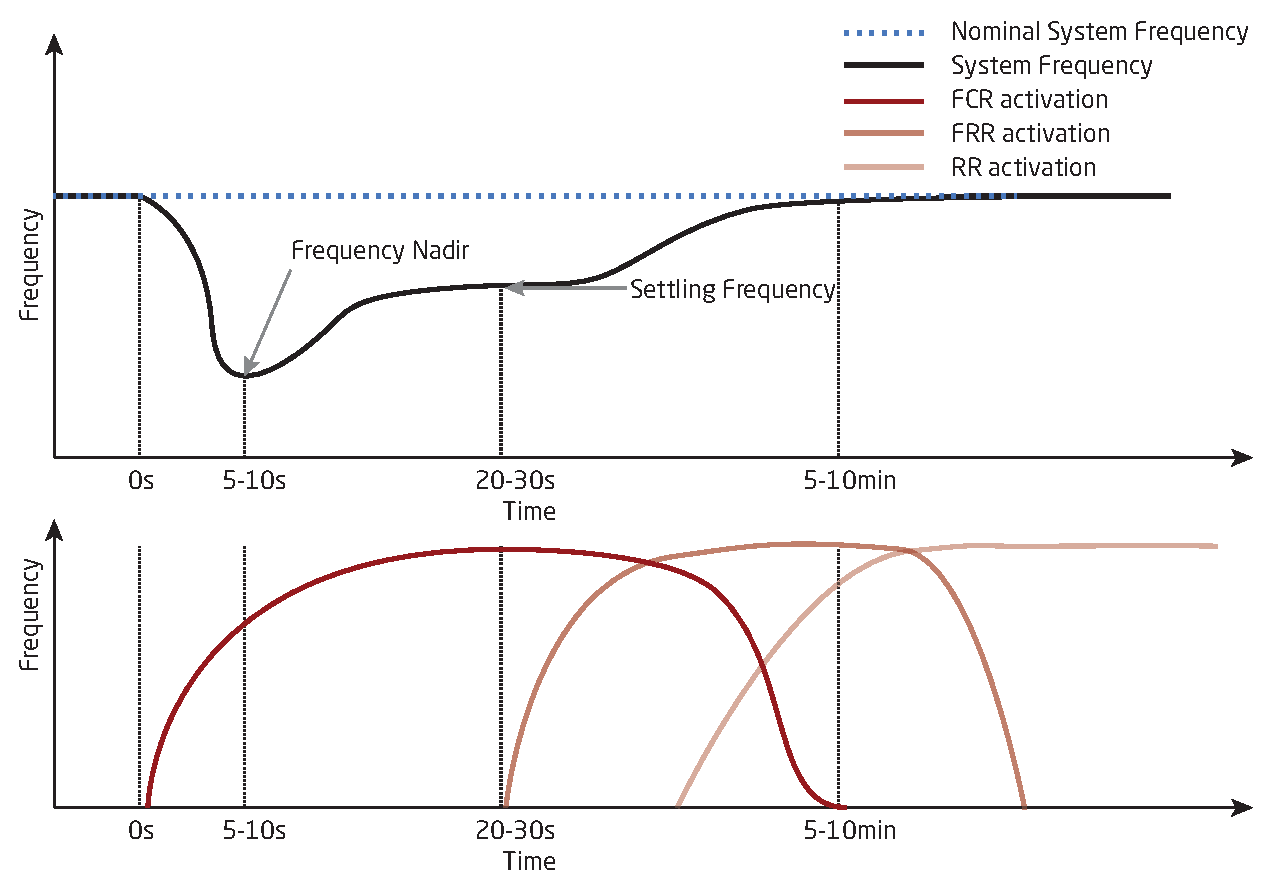
\includegraphics[width=1\columnwidth]{frequency_contingency.eps}
\caption{The nadir of a system frequency excursion during contingency events is more pronounced if there is less inertia in the system.}
\label{fig:contingency}
\end{figure}

\subsection{Ancillary services}
The objective of ancillary services can generally be defined as: maintaining an adequate and secure power system. This means maintaining the power system operating at nominal frequency and voltage. In cases where the power system deviates from nominal operation, either due to natural fluctuations in consumption or faults in the system, the system operators will activate ancillary services to restore normal operation.

Power produced by renewable energy sources (RESs) has a low marginal price, which pushes the overall electricity prices down in markets with high RESs penetration. This means that the operation of traditional generators is becoming economically challenging, and will lead to the decommissioning of fossil-fueled generators. In other instances the regulatory framework prioritizes renewable production, which also leads to the decline of fossil-fueled generators\cite{eurelectric2015sector}. Both cases lead to a system with less inertia and leaves the system operators with fewer sources for ancillary services. New sources of ancillary services will become important, and it is in the interest of the system operators that the remaining sources for ancillary services, both from production and consumption sides, are exploited optimally.

\subsection*{Primary Frequency Control}
Primary frequency control is the fastest response (in the seconds range) and is used to arrest and begin reversing frequency excursions occurring due to sudden imbalances between supply and demand, often caused by contingency events. Primary frequency control is traditionally performed by generators under ``droop'' control, in which a  change in power output is made proportional to locally measured frequency. The reason for this is that the response to the frequency excursion must occur as fast as possible and be proportional to the size of the excursion so that the system frequency stabilizes within an acceptable time frame.
\subsection*{Secondary Frequency Control}
Secondary frequency control is a slower response (in the seconds to minute range) that takes over for the primary frequency control and returns the system to nominal frequency by controlling the output of participating resources. Much more urgently, it restores the full bipolar range of the primary reserve, so the system gets back to nominal $n-1$ redundancy. Usually an entity estimates the control reference signals based upon the ACE and system frequency to simultaneously resolve the imbalance at the interconnection and maintain stable operation (see, e.g. \cite{nerc2011balancing,entsoe2014continental}, for more details). The control algorithm that directly controls the output of resources providing this service is often called Automatic Generation Control (AGC)\footnote{This balancing control logic can have a centralized, pluralistic or hierarchical architecture~\cite{entsoe2014continental} to determine the individual reference signals for the generators.}. The generators will have either a proportional controller or a proportional-integral (PI) controller to track the AGC signal. The secondary response also needs to occur as fast as possible, yet due to its centralised control approach, it is not able to provide as fast a response as primary control. The underlying need for the secondary service is to supply a fast reference tracking response without overshoot.

\subsection*{Service Requirements}
Because AS are essential for the secure operation of the system, the system operators also have requirements and restrictions on the units providing AS. A super-set of requirements across different systems is defined in \cite{Rebours}. These requirements can roughly be classified into three categories: \emph{temporal requirements}, which relate to how fast and for how long a service must be delivered; \emph{resource tuning requirements}, which relate to specific values that tuning parameters in the resource must have; and \emph{market requirements}, which relate to bid sizes and similar parameters in systems where services are acquired through market mechanisms. Of these three categories, only the temporal requirements relate to service performance. Furthermore, in most systems are the requirements implicitly defined for traditional generation units. This means that most service requirements are oriented towards the least common denominator of service providers, e.g. a unit providing primary frequency control should provide half of the service within 15 seconds and full response within 30 seconds\cite{EnerginetAncillary}. A variety of generation and consumption units would be able to provide this service faster, but this quality is not rewarded. Another example is the requirement of having a PI-controller on units providing secondary frequency control, in order to track the AGC signal. Such a controller is infeasible on distributed systems, but other modern controllers can provide offset-free control with similar properties.

%Units which do not perform within the specified requirements are heavily fined. \macd{I assume there will be more to follow this statement?}\bondy{Yeah, I had hoped you might want to write a line or two here :-).}

\subsection{Problem statement}

 Until now, system operators have been able to arrest frequency excursions fast enough because of the inherent system inertia, but as the inertia decreases, faster response times are required of the primary frequency control.

The system operator must have enough primary reserves to arrest the frequency as fast as possible, before the system enters a state where a blackout is inevitable. A metric for how effective the procurement of reserve is the \emph{frequency nadir} \cite{eto2010use}, and it is desirable that the value is as close as possible to the nominal frequency of the system.

Similarly, the system operator should ensure that the secondary reserves act as fast as possible to relieve the primary reserves and also bring the frequency from the settling frequency back to the nominal frequency.


In \cite{vrettos2015integrating} it is shown that if primary frequency response is provided by demand response (with a very fast response), the frequency nadir occurs at higher frequencies.
Also, in \cite{makarov2008assessing}, the authors argue that the value of regulation resources can be defined based upon the ramp capabilities of the service providing units. Faster reacting units are more valuable to system operators, since they help arrest the frequency excursion faster and at a higher nadir. It does require changes to the AGC in order to utilize the fast response, but this would also lead to the need for fewer reserves.

In short, the historical definitions for service requirements results in the suboptimal use of today's AS resources. Due to the legacy definitions there is an implicit %explicit
bias for traditional resources, and alternative technologies, such as demand response, are are restricted in their contribution to AS provision, and their favorable properties are not utilized or undervalued.

While system operators have been able to maintain a secure system using traditional resources, the changes in the power system, i.e. the decrease of system inertia and increased fluctuation due to RES, require units that react faster than the current minimum requirements. Also, an increased overall volume of balancing resources will be required due to the larger deviations caused by the RES.
Units that provide a faster response but are not able to provide the full response duration should be enabled to contribute to AS provision and be valued accordingly.

If these technologies, both the underutilized and the ones restricted from providing services, are used optimally for ancillary service delivery, it follows from the conclusions presented in \cite{makarov2008assessing,vrettos2015integrating} that frequency excursions could be arrested at higher frequency nadir, thus lessening the required amount of reserves, which leads to a lower-cost operation of the system.
Regulative authorities have concluded that fast reacting units are valuable for the system operation, and started programs to benefit of these resources. An example of this is FERC order 755 (Pay for Performance) which has led to PJM splitting their regulation market product into RegA, for slow reacting units, and RegD for fast reacting units. The product differentiation approach has been a success for PJM, but splitting the market into different products does not address two points: 1) the overall pool of resources will not be optimally utilized, and 2) as other new technologies appear in the system, the market might fragment further, also leading to non-optimal utilization of resources.  We propose instead to restructure the ancillary service definitions such that all types of service providers participate with the same market product defined by a set of optimal performance parameters, and not by minimum requirements. This means that the all entities providing a given ancillary service, e.g. primary frequency control, are optimally cleared under a single market. The service restructuring is detailed in the following section.


\section{Unconventional Resources}
\label{sec:ancsrvDR}

\subsection{Related Work}
There is growing evidence that demand-side resources (DSRs) can participate in ancillary services, thus substituting the need for traditional ancillary service resources. However, the DSRs that can provide ancillary services vary greatly in composition, and have distinct properties. Most of the research on DSRs to provide transmission-level services has focused on specific services using a particular set of loads connected to the grid. This is partly due to varying characteristics of DSRs and partly to the suitable control architecture for the proposed services. 

A common set of resources studied in connection to DR are thermostatically controlled loads~\cite{Molina_Garcia_2011,Kara_2012,thavlov2014utilization,mathieu2012using}, such as electric space heating \cite{mathieu2012using,thavlov2014utilization}, residential and industrial refrigeration \cite{lakshmanan2014energy}, and space heating using heat pumps \cite{halvgaard2012economic}. Thermostatically controlled loads are valued for their ability to provide ancillary services because of the inherent thermal inertia present in the systems. The thermal inertia acts as energy storage, permitting the curtailment or deferral of power consumption. The application of TCLs as a DR mechanism can also be seen in industrial settings such as large refrigeration systems \cite{rahnama2013integration}, the heating of bitumen tanks \cite{cheng2014availability}, and indoor climate control using HVAC \cite{blum2013ancillary}. 

Batteries can also provide ancillary services through demand response. Electric vehicles (EVs) can be considered as mobile batteries with additional time varying constraints. By changing their charge patterns while guaranteeing the mobility needs of the owner, EVs can offer the demand-side flexibility needed to provide ancillary services to the grid \cite{zarogiannis2014dynamic,kara2015estimating}. 

The potential of using the dimming of lighting in office buildings for DR is presented in \cite{rubinstein2011demand}. A pilot project in Denmark also used the lighting system in an industrial green house for DR, showing the potential of using DR to manage congestion in the distribution system. 

Water pumps--used in wastewater treatment systems and agriculture--are also considered a promising resource for ancillary services. Specifically, in \cite{halvgaard2014waste}, the authors suggest that water can be temporarily stored in pipes and tanks, hence delaying the transportation for treatment in waste water treatment systems. The load flexibility of agricultural water pumps stems from the inherent flexibility in the time of irrigation.
%The response of the pumps is fast, and depending on the system state and weather conditions can be sustained from medium to long time. The system requires a certain amount of energy to move the water around, and is therefore deferrable. Due to the pumps there may be constraints on the cycling.
%Furthermore, 50\% of the energy consumption of a waste water treatment plant is spent on the aeration process, which can also be deferred. 

In this paper, we examine the use of DR when system reliability is jeopardized. A great deal of research has focused on DSR-specific controller design and limitations due to load characteristics and comfort needs. Specifically, many aggregation frameworks exist in the literature that overcome cycling constraints and response frequency limitations. Hence, instead of focusing on the design of such DSR-specific controllers, we assume that AS provided by DSRs will be sold to system operators by an aggregator, and that the aggregator is responsible for control accuracy. 
Our objective in this paper is to discuss and formulate ideal performance requirements for ancillary services in a number of relevant features, and to provide a market clearing mechanism that selects a portfolio of resources in a resource-agnostic and performance-oriented way. By doing so, we propose a strategy in which (i) we remove the barriers preventing unconventional resources from participating in AS markets due to the static nature of AS market definitions and requirements, and (ii) we provide a fair and performance-based market clearing structure in which the unused potential of DSRs can be easily incorporated.

\subsection{Properties}
The identified DSR parameters are given as follows:
%\kara{I think here we need a discussion of parameters that we are using in Section 4 to define $\kappa$} \kara{I think the properties should be of aggregations, not necessarily the DR resources}
%\olge{I know I probably spend way too much time looking at microcontroller timing diagrams, but would it help trying to put all the parameters into a single timeline drawing like the sketch in figure {\ref{fig:resourcecharacteristics}} ?}
%\begin{figure}[htb!]
%\centering
%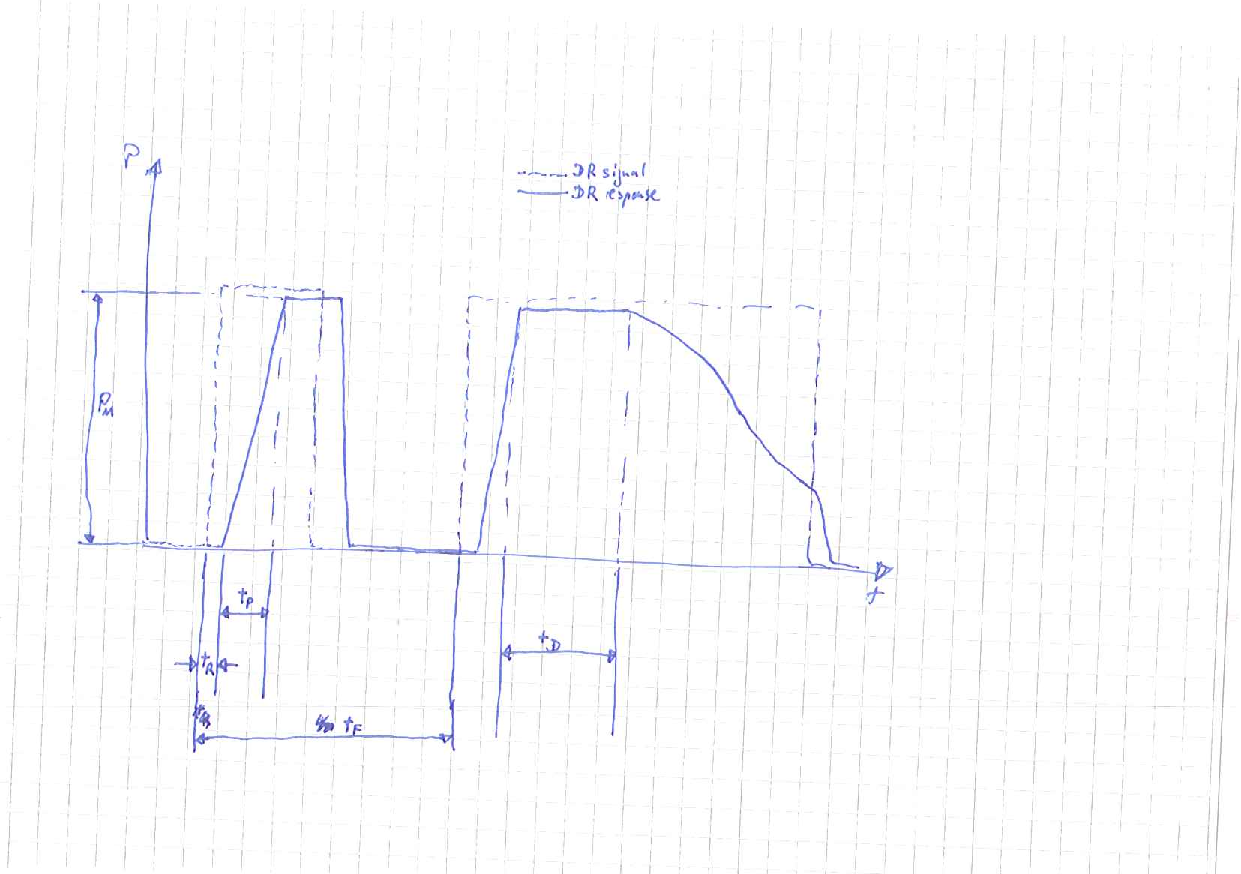
\includegraphics[width=1\columnwidth]{20150731150249153.pdf}
%\caption{Characteristics of demand side resource [sketch].}
%\label{fig:resourcecharacteristics}
%\end{figure}

\begin{description}
    \item[Response time] This is the time it,takes for a unit to receive a DR signal and react upon it. %\textcolor{red}{I'm not sure on this one, since pretty much all of them have fast response time, depending on the control architecture and the communication system, which are not inherent to the DER}
    \item[Response duration] How long is a pool of these units able to sustain service provision: short, medium or long. %\textcolor{red}{Again, this is a tough one, since this will depend on the state of the portfolio/unit}
    \item[Response magnitude] This the \emph{amount} of load used by the DR resources that can be increased or decreased. The increase capability is defined as the \emph{take} magnitude and the decrease capability is defined as the \emph{shed} magnitude.
\end{description}


\subsection{Unused Potential of DSRs and Barriers to DSR Participation}

\label{subsec:unused}
Although DSRs provide additional freedom to help shape response compared to traditional AS providers, the existing ancillary service market rules and requirements are a strong barrier to DSR market participation. A recent study identifies such barriers in the US\cite{cappers2013assessment}. The rules and requirements that limit resource participation in different markets are not consistent among different RTOs and ISOs; however, the authors identify three major groups of these rules: rules on the size of the resource, rules on the measurement and telemetry of the resource, and rules on market bidding time. Out of six different ISOs and RTOs in the US, only one allows load aggregations to provide regulation services, and only two allow aggregation participation as a spinning reserve provider. Furthermore, only two ISOs and RTOs allow aggregate telemetry. Providing telemetry at an individual resource level increases the overall cost of metering, making it challenging for DSRs to provide cost-competitive AS. Finally, most of the AS markets procure in day-ahead markets, and day-ahead DSR participation is harder due to increasing uncertainty in DSR flexibility forecasts.  

In order to accommodate the slow-ramping resources as well as DSRs in the AS markets, there is an increasing need to either split AS into different service classes or parametrize the service definition so that the resources are selected only by their ability to satisfy the system needs. The ideal resource to satisfy the system need is one with ``unlimited capabilities in terms of response time, energy output, ability to frequently reverse their output, ability to respond and follow the AGC setpoint changes, and size.''\cite{makarov2008assessing}\footnote{For this kind of response to be optimal, changes must be made to the AGC algorithm \cite{peydayesh2012effects}.} To include and incentivize the participation of technologies that in some parameters are closer to the ideal than those defined by the current service and market requirements, two methods can be utilized: product differentiation and product restructuring.

Some transmission system operators, like PJM, have already suggested that better service performance is more valuable than simply adhering to traditional rules and requirements, and split their regulation market into a slow service product and a fast service product. 
This work explores the alternative: restructuring the market so that all technologies can participate in the same market, and the system operator can optimize the use of the resources based upon their capabilities. This entails reformulating the temporal and market requirements, and removing the requirements that implicitly assume that the services are provided by traditional generators, thus making the requirements technology-agnostic. %In the next section, we discuss the \emph{new proposition}.\kara{to be filled} 


 

\section{Restructuring the Ancillary Service Requirements}
\label{sec:newas}
\subsection{Overall approach}
%[argument vs. current approaches start supporting performance of new resources by a more lenient apporach blb bla cut it]
%\kh{Guys, we really have to clarify the workding of 'performance': in performance-based remuneration, the 'performance' is a 'quality of execution' (Sect. 4.4 $\eta^{AS}$); however, our $\kappa$ does not look at 'performance' but rather at a 'quality of shape' (lacking a better word to describe the 'fitness' assessment quantified by $\kappa$.)}

%The key idea of the proposed approach is to formulate ideal performance requirements for each ancillary service in a number of relevant features, and then to provide a market mechanism that allows to define an optimal control resource portfolio building on beneficial combinations accounting for complementary properties of control resources. 
The proposed restructuring assumes that system operators acquire AS reserves through a market, and that potential AS providers bid their reserve capacity in that market. The restructuring is based on the following four key concepts (which are expanded upon throughout this section):
\begin{itemize}
    \item The formulation of an \emph{ideal ancillary service response} that the system operator desires for the system. This formulation will be strongly dependent on the needs of the system operator, e.g. very fast response in case of low system inertia, and will be submitted as a tender to the market.
    \item The \emph{parametrization of the AS bids}, where the parameters reflect the service providers' capabilities to partially fulfill the ideal service response. This removes the minimum-requirements-barriers on new technologies, thus enabling any useful unit to participate in the AS provision, which facilitates market liquidity.
    \item Clearing all units under a \emph{generalized single clearing-price auction}, provides incentives to bid actual marginal cost. In this auction, the capability value of each service provider and their historical performance is taken into account.
    \item \emph{Performance-based remuneration} gives incentive to better AS provision and enables transparent performance-based clearing of the market.
\end{itemize}

Based on an assessment of the complete decision process, we merge the four key concepts outlined before into a novel approach to an ancillary service definition that accounts both for performance of resources and the actual spectrum of system needs.  % The actual market clearing is then
The holistic assessment includes:
\begin{itemize}
	\item \textit{Planning}: Assessment of system need, parametrization of resource performance and specification of tender conditions.

	\item \textit{Scheduling}: Quantification of AS tender volume, AS bid submission, and market clearing.

	\item \textit{Operation}: Reserves dispatch/activation and monitoring.

	\item \textit{Settlement}: Verification of service delivery and remuneration.
\end{itemize}

As outlined above, for effective inclusion of DR (or any other unconventional resource) in AS markets, a revision of each phase is required. Our proposal focuses on a new \textit{parametrization of services} (Sec.~\ref{subsec:parametrization}), which affects in particular \textit{market clearing} (Sec.~\ref{subsec:marketmechanism}) and \textit{remuneration} (Sec.~\ref{subsec:performanceremuneration}). 

In Section~\ref{sec:ddrascasestudy} we illustrate the impact of this reformulation in comparison with present market mechanisms, and in \ref{sec:ddrasdiscussion}, the alignment with present mechanisms and its applicability to novel ancillary service models (REF WARRINGTON/policy based) is reflected.  

\subsection{Ideal service tender}\label{subsec:idealtender}
The ideal source for AS is one with ``unlimited capabilities in terms of response time, energy output, ability to frequently reverse their output, ability to respond and follow the AGC setpoint changes, and size .''\cite{makarov2008assessing}\footnote{For this kind of response to be optimal, changes must be made to the AGC algorithm \cite{peydayesh2012effects}.} It is impossible for any one unit to possess these characteristics, but system operators aim at achieving this kind of system response by contracting several units.

In existing AS, there is an implicit assumption that ideal unit response corresponds to a scalar fraction of the required system response. In contrast, in presence of a diverse resource portfolio, the commonly expected fast response is secondary to an overall cheaper mixed portfolio which delivers a better system response, e.g. by combination of a fast duration-limited and slower unlimited response time resources.

%\kh{What is the difference between conventional dimensioning (see "operations manual") and dimensioning with capability parametrization?}

For example, a system operator could determine that the ideal system response to a frequency excursion is the one that has a resulting frequency nadir at the settling frequency (thus minimizing the risk of tripping the under-frequency relays). Based upon the inertia in its system, the system operator determines the volume ($V_{tot})$ needed as well as the response characteristics needed to achieve this, see Figure~\ref{fig:ddrasidealresponse}.

\begin{figure}[htbp!]
\centering
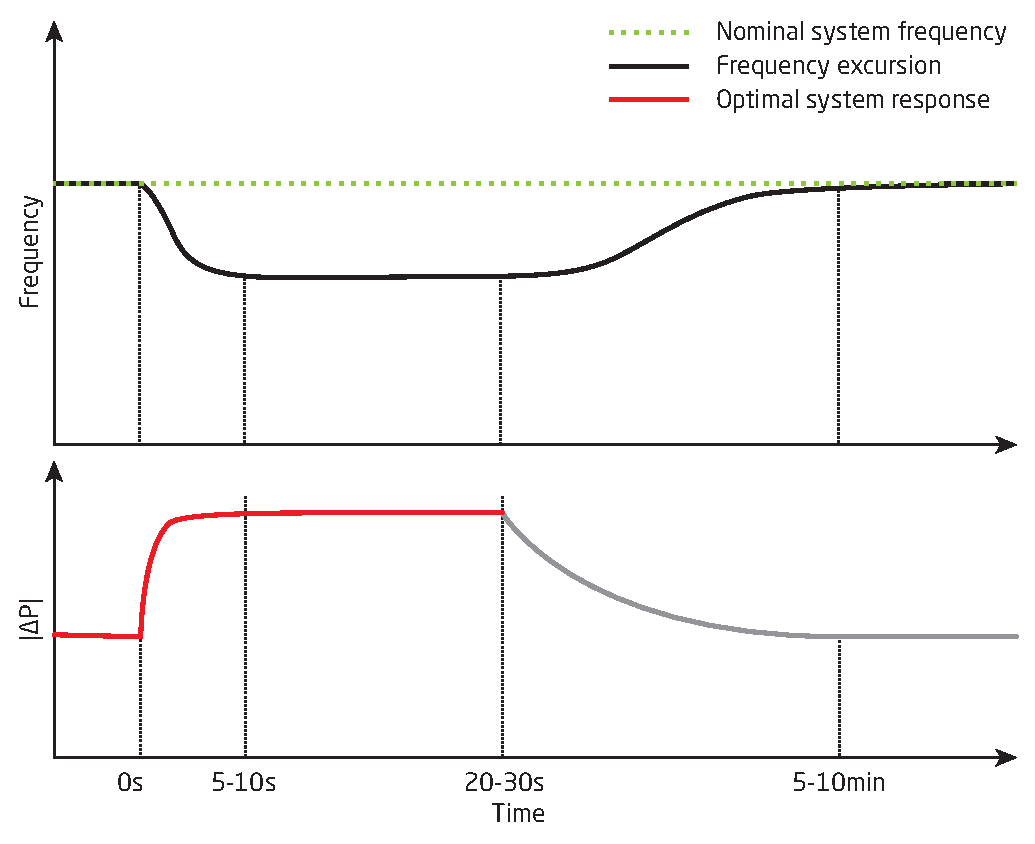
\includegraphics[width=1\columnwidth]{graphics/ddras/primary_frequency_control_ideal.eps}
\caption{In this case, the ramp of the ideal response is mainly determined by the system inertia and is to be sustained until secondary frequency control can be activated.}
\label{fig:ddrasidealresponse}
\end{figure}
%%4.2
%* bid formulation uses simplified constraints that can be addressed both for conventional generation and are also straightforward to be formulated as response capability of a diverse DR portfolio;

\subsection{Parametrization of service performance}\label{subsec:parametrization}
Ancillary service requirements are specified by a system operator based on the desired control response for a particular power system. Today, these requirements --- as reflected in the service definition --- are not differentiated according to the capabilities of the unit providing the service. Therefore, service definitions are designed to accommodate the least capable unit in the portfolio. As a consequence, more capable units are not being fully utilized, leading to excess contracting of service providers.
This suboptimal allocation of resources could be addressed by introducing a performance dependent definition of ancillary services, i.e. a service definition which allows compliance to be measured on a linear rather than a binary scale: In addition to compliance and noncompliance, different levels of partial compliance are possible.
In this context, services will be defined such that the best possible performance of the most capable unit corresponds to full compliance.

One of the challenges with such an approach is to achieve a useful definition of partial compliance. Depending on the complexity of the service, many parameters of DR resources may have to be included in a performance comparison to determine their relative value. For example, resources with identical response magnitudes, ramp rates and endurances may represent a significantly different value to the buyer of a cyclic service if one resource requires a high recovery time between cycles. A performance model is therefore needed to provide a mapping between the multidimensional parameter space of a DR resource and its capability to comply with a given service, expressed on a linear scale. 

We introduce the following definition of a capability value:
\begin{align}
    \kappa &= g(\mathbf{x}) \\
    \kappa &\in [0,1]
\end{align}
where $\mathbf{x}$ is a vector of the resource parameters relevant to a particular service, and $g(\cdot)$ is a function mapping the parameter space to a scalar value according to resource utility. This mapping function is highly specific to a particular service and must therefore be developed by the service requester, e.g. a TSO. The function is then communicated to the resources as part of the service definition included in a tender. $\kappa$ for a particular resource can then be calculated by its operator prior to bidding.

%%4.3
\subsection{Market mechanism}\label{subsec:marketmechanism}

In order to leverage the proposed AS restructuring, the market clearing mechanism needs to be changed. The clearing should take the \emph{capability value} of the service providers into account, and ideally also the probability of availability (certainty in service). There are many different ways of formulating such a market clearing mechanism and here we present an example of a market that utilizes the service parametrization to form an ideal service response.

The market is designed as a single clearing price auction, in which each resource bid is adjusted by \textit{two} factors for bid quality: 1) a shape-matching parameter $\kappa_i$ and 2) a historic performance  parameter $\eta^{hist}_i$.
%The benefit of the merit order is that by remuneration at clearing price it provides competitive incentive for bidding with true marginal cost 
The clearing mechanism identifies a common clearing price based on the most expensive accepted bid. 
%Clearing principles
\begin{equation}
    P^\mathtt{clear} = \max P^\mathtt{bid}_i, \quad i \in \Omega^\mathtt{acc}
\end{equation}
where $\Omega^{acc}\subseteq \Omega$ is the subset of accepted bids of the set of received bids $\Omega$. 
The clearing mechanism selects the subset of bids which offer the cheapest overall clearing cost and meet the tender requirements: 
\begin{align}
      \Omega^\mathtt{acc} &= &\mathtt{argmin}_{\Omega^\mathtt{hyp} \in \mathcal P(\Omega)} \sum_{i\in \Omega^\mathtt{hyp}}{\kappa_i P^\mathtt{clear}_{\Omega^\mathtt{hyp}} } & \\
      &\mathtt{s.t.}& \sum_{i\in \Omega^\mathtt{hyp}} V_{i}\ge V_{tot} &  \\
      &~ & \eta^{hist}_i \geq \eta^{hist}_{min} &\quad \forall i \in \Omega^\mathtt{hyp} \\
      &~ &\sum_{i\in \Omega^\mathtt{hyp}}{\eta_i V_i}/V_{tot} \geq \eta^{AS}& 
\end{align}
Where $\mathcal P(\Omega)$ denotes the Power Set of $\Omega$.
%As both tender specification and bid parametrization correspond to a $n$-dimensional polygons, the bids can be summed up and the sum can be compared to the tender polygon.

The specification of tender and bid parametrization needs to be aligned with the mechanisms applied during real-time operation the resource dispatch and activation.
Resource performance is monitored with respect to the behaviour expected from bid parametrization, and is further expanded upon in the next subsection.




%%4.4
\subsection{Performance-based remuneration}\label{subsec:performanceremuneration}
%\bondy{I write here}

%\bondy{3) adherence to performance model is evaluated and applied to base price}

Performance-based remuneration has already been introduced in United States through the FERC order 755. Similarly, in this work we propose that service providers are paid according to how close they follow the capability parameters they bid to the market. The estimation of the service provision performance can be done in different ways, depending on which parameters the system operator deems to be the most critical. A service performance index is proposed in \cite{bondy2016method}, where service performance is defined as the root mean square error of the actual service delivery compared to the ideal model:
 \begin{align}
     \eta^{post} &= \sqrt{\frac{\sum^{N}_{t=0} \left( {QoS_{t}}^{2} \right)}{N}},\\
     \eta^{post} & \in [0,1],
 \end{align}
 where \emph{N} is the time horizon over which the service is delivered and $QoS \in [0,1]$ is the \emph{Quality of Service} of the ancillary service, which is the error in service delivery scaled to the tolerance limits defined by the system operator. This leads to the final settlement price of service provision being defined as:
\begin{equation}
    P^\mathtt{rem}_i = \eta^{post}_i\kappa_i  P^\mathtt{clear} \qquad \forall i \in \Omega^\mathtt{acc}.
\end{equation}
 


%\section{Case study}
%\label{sec:newas}
%Using two different ancillary services and an asset management service as cases, we will illustrate the utility of the generic service modeling method, the service performance index and the service verification index. The first case study focuses on frequency containment reserve in western Denmark, the second focuses on the theoretical PowerMax DSO service, and the third focuses on the temperature management of a residential house. 

\subsection{Frequency Containment Reserve in Western Denmark}
Frequency Containment Reserve (FCR) is utilized to contain frequency excursions deviating from the nominal 50 Hz in \emph{ENTSO-E RG Continental Europe’s synchronous area} of which western Denmark (DK1) is part of. The Danish TSO, Energinet.dk, is obliged to provide a proportional share of $\pm$ 23 MW \cite{EnerginetAncillary} out of the total synchronous area need of $\pm$ 3000 MW. Energinet.dk buys these reserves at daily auctions. The service specifications are defined in \cite{EnerginetAncillary}.

The six steps outlined in Sec.~\ref{sec:SEGANmethodology} are used to model the ideal and tolerated service response. 1) The physical parameters are grid frequency (accuracy of $\pm$ 10 mHz or better), generator reserve power output, and timing of service delivery (accuracy of 1 s or better). 2) The reserve must be supplied linearly at deviations of $\pm$ 200 mHz relative to 50 Hz, with a $\pm$ 20 mHz dead-band around 50 Hz. 3) The physical size of the service depends on the reserve bid size. This work will look at a generic reserve bid. According to the discussion from Eq.~\eqref{eq:QoS}, $x_{ideal}$ cannot be equal to $\mathbf{x}_{acc}$. Therefore, a $\pm$ 1\% tolerance band of $x_{ideal}$ is assumed. 4) The first 50\% of the service must be supplied within 15 s and 100\% must be supplied within 30 s. The ideal response can be defined as a response with an instant 100\% power ramp \cite{makarov2008assessing}. 5) The ideal and tolerated response of this service provision is plotted as $x_{ideal}$, $x_{acc,min}$ and $x_{acc,max}$ in Fig.~\ref{fig:DK1PrimResSim}, which assumes that a reserve power set-point has already been established based on the values from step 2.%Fig.~\ref{fig:DK1PrimResDyn}

%\begin{figure}
%\centering
%\includegraphics[width=\columnwidth]{figures/dynresp.eps}
%\caption{DK1 Primary Reserve service provision curve. The curve shows the relationship between the activated fraction of the primary reserve bid, and the grid frequency, including the +/- 20 mHz dead-band. This should not be confused with the droop curve.}
%\label{fig:DK1PrimResDyn}
%\end{figure}

Fig. \ref{fig:DK1PrimResSim} shows a simulation of primary regulation active power ramp $x_{act}$ for the time interval $[-5,35]$ s. The service delivery performance index and non-delivery verification index are $\eta^{AS}=0.4257$ and $\epsilon^{AS}=0.1392$, calculated using Eq. \eqref{eq:etaAS} and Eq.~\eqref{eq:epsilonAS}. The TSO must determine a threshold $\epsilon_{max}$, such that the service provider is penalized or the contract is terminated if $\epsilon^{AS}>\epsilon^{AS}_{max}$. It is not the scope of this work to asses a suitable value of $\epsilon^{AS}_{max}$.%\bondynote{We are repeating ourselves a bit here}

\begin{figure}
\centering
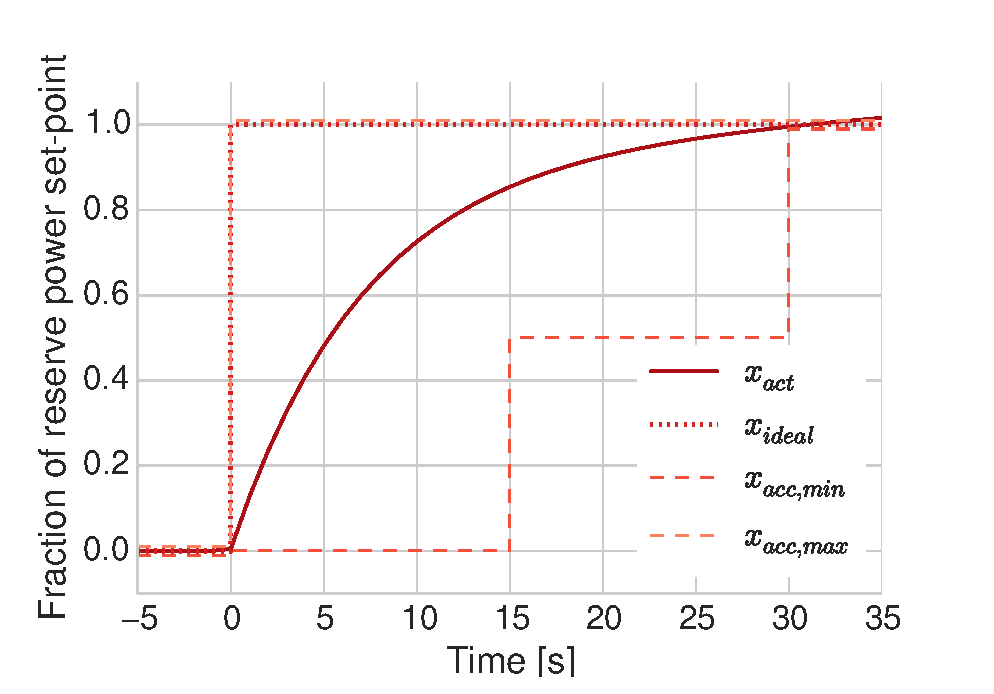
\includegraphics[width = \columnwidth]{SEGAN/primfreqresp.eps}
\caption{Simulation of a DK1 primary reserve power ramp response together with $x_{ideal}$ and $x_{acc}$ values.}
\label{fig:DK1PrimResSim}
\end{figure}

\subsection{PowerMax in a distribution system}
The \textit{PowerMax} service was first described in \cite{ding2013development} and further specified in \cite{bondy2014flech}. It is a DSO service, where the DSO can make a tender for a load reduction $\Delta P^{DSO}$ to a max level $P_{max}^{DSO}$ in parts of the distribution system that are forecasted to experience congestions during some periods (e.g. hours 17-20 during winter months). The motivation for \textit{PowerMax} is that the service could be an economically beneficial alternative to grid reinforcements in some situations. This is both due to saved interest and depreciation on investments plus the avoided risk of over-sizing equipment in case of future energy savings or if the disappearance of a large consumer makes the reinforcement unnecessary.% The tender is announced and cleared through Flexibility Clearing House (FLECH), where flexibility aggregators can bid on the tender.%where the service is delivered by aggregator companies, which bid in flexibility from a group of units which they control. 

%Following is a mathematical definition of the \textit{PowerMax} service, as previously developed in \cite{bondy2014powermax}. 
In order to identify its service needs, it is assumed that the DSO is able to separate the total consumption forecast $\hat{P}_{tot}$ in the congested part of the distribution grid into a controllable load forecast $\hat{P}_{CL}$ and a base load forecast $\hat{P}_{BL}$:
\begin{align}
\hat{P}_{tot} &= \hat{P}_{CL} + \hat{P}_{BL} \\
\hat{P}_{CL} &= \sum_{Agg} \hat{P}_{CL,Agg}, \quad Agg \in \mathbf{A} \label{eq:CLDef}
\end{align}
where $\mathbf{A}$ is the set of all aggregators in the considered part of the grid. Only the aggregators \emph{Agg} that bid for the service tender make up $\hat{P}_{CL}$, while the rest of $\mathbf{A}$ is part of $\hat{P}_{BL}$. The aggregators must be contracted to deliver a total power reduction $\Delta P$, such that the system operational limit $\bar{P}_{sys}$ is not violated by the peak base load forecast and the peak controllable load forecast:

\begin{equation}
\hat{\bar{P}}_{BL}+\hat{\bar{P}}_{CL}-\Delta P \leq \bar{P}_{sys}. \label{eq:PSysDef}
\end{equation}

This inequality can be fulfilled by setting a peak limit $\bar{P}_{CL}$:
\begin{equation}
\bar{P}_{CL} = \hat{\bar{P}}_{CL} - \Delta P \label{eq:PBarCLDef}
\end{equation}
where $\Delta P$ and $\bar{P}_{CL}$ are the variables for the DSO service tender. In order to formulate a service tender, the magnitude of these variables must be estimated taking into account the uncertainty of the forecasts, giving the following expressions:
\begin{align}
\Delta P^{DSO} &= \sum_{Agg} \Delta \hat{P}_{CL,Agg} + \text{Risk\{}\hat{P}_{CL} + \hat{P}_{BL}\text{\}}\\
P_{max}^{DSO} &= \hat{\bar{P}}_{CL} - \Delta P_{DSO}
\end{align}
where $\Delta \hat{P}_{CL,Agg}$ is the estimated power reduction for the individual aggregator bid, $\text{Risk\{}\hat{P}_{CL} + \hat{P}_{BL}\text{\}}$ is the risk associated to the load forecast uncertainty. $Agg \in \mathbf{A_{C}}$ and $\mathbf{A_{C}} \subseteq \mathbf{A}$, i.e. $\mathbf{A_{C}}$ is the subset of aggregators that bid on the tender. After the DSO has identified a suitable $P_{max}^{DSO}$ and $\Delta P^{DSO}$ to solve the congestion issue, the DSO formulates a service tender for which aggregators can bid their corresponding $\Delta P^{Agg}$ and $P^{Agg}_{max}$. %The DSO sets a maximum price it is willing to pay for the load reduction, which is related to the alternative cost of grid reinforcements. In case the market is not cleared at or below the maximum price, the DSO can formulate a new tender, adjusting the risk value, POD (point of delivery) list or amount of power reduction. The timing of the tender process should be such that the DSO has time to conduct grid reinforcements as an alternative.

The method from Sec.~\ref{sec:SEGANmethodology} is used to model \textit{PowerMax} ideal and acceptable response. 1) The physical parameters are $P_{max}^{Agg}$, $\Delta P^{Agg}$ and months/days/hours the service shall be delivered. 2) The system does not posses a dynamic behaviour related to system parameters. 3) As an example, the service tender defines $P_{max}^{Agg} = 200$ kW and $+1\%$ allowed deviation $P_{max,acc}^{Agg}$. 4) In this example we use 120 min service provision time with allowed non-delivery in the first 15 min, and the last 5 min, of the service delivery (following the service definition in \cite{ding2013development}) and the ideal service delivery is the one that respects $P_{max}^{DSO}$. 5) Figure \ref{fig:PowerMaxSim} plots $x_{ideal}$ and $x_{acc}$. The \textit{Activation Dead-band} indicates the regions where the aggregator is not obliged to deliver the service because of the tolerances defined under step 4. 6) The service is a maximum cap service and the error is measured as in Eq.~\eqref{eq:maxmin_cap}.

An example of a load curve $P_{Agg}=x_{act}$ is presented in Fig.~\ref{fig:PowerMaxSim}. The service delivery and verification are evaluated using Eq.~\eqref{eq:etaAS} and Eq.~\eqref{eq:epsilonAS}, yielding $\eta^{AS} = 0.5074$ and $\epsilon^{AS} = 0.2701$ respectively. As with the performance assessment of the FCR in DK1, it is not within the scope of this paper to asses the value of $\epsilon^{AS}_{max}$, yet a qualified assessment can be made. %, which will lead to either penalization or termination of the contract.
To asses $\epsilon^{AS}_{max}$, the DSO must analyze the dynamics of the problem the service is helping relieve. For \textit{PowerMax}, the dynamics are governed by the heating of the overloaded equipment (e.g. transformer or cable), which deteriorates over time due to overheating. A feeder might be tolerant to short term overloads and therefore the DSO might set $\epsilon^{AS}_{max}$ higher than in the FCR case.

\begin{figure}
\centering
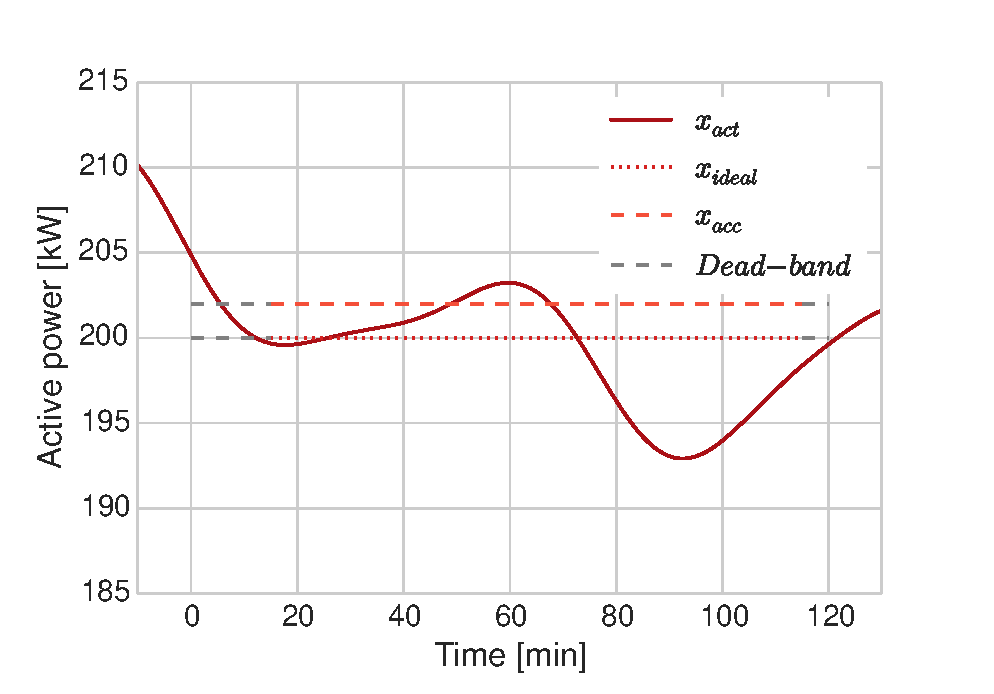
\includegraphics[width = 0.86\columnwidth]{SEGAN/powermaxsample.eps}
\vspace{-4pt}
\caption{$x_{ideal}=P_{max}^{Agg}$, $x_{acc}=P_{max,acc}^{Agg}$ for the considered \textit{PowerMax} example. The activation Dead-band is the time period, where the aggregator is allowed to non-deliver.}\label{fig:PowerMaxSim}
\end{figure}

\subsection{Temperature management of a flexible household}
Household heating is a flexible process where the thermal capacity of the building can be considered a form of energy storage. In Denmark, heat pumps are being installed with the capability of being remotely controlled by an aggregator, see e.g. \cite{insero}. It is assumed that the aggregator will help the heat pump owners to maintain a comfortable indoor temperature and utilize the electric consumption flexibility in exchange of monetary compensation.

Applying the method from Sec.~\ref{sec:SEGANmethodology} to model the service: 1) The physical parameters are the minimum and maximum of the temperature comfort bands of the household. 2) The service does not posses a dynamic behaviour related to system parameters. 3) As an example, the household owner sets a comfort band of $\mathbf{x}_{ideal} = [x_{min},x_{max}] = [20 ^{\circ}\text{C},22^{\circ}\text{C}]$ and allows for a $\pm 1 ^{\circ}\text{C}$ as acceptable error. Furthermore, the owner decides that during the night, the house can be two degrees colder. 4) In this example the ideal response is performance within the temperature bounds. 5) Fig.~\ref{fig:tempband} plots $x_{ideal}$ and $\mathbf{x}_{acc}$. 6) The service is a band service and the error is measured according to Eq.~\eqref{eq:band_error}.

The service model and the actual temperature of a simulation can be seen in Fig.~\ref{fig:tempband}, where it is clear that generally the aggregator is able to provide a reasonable service performance, with no non-delivery ( $\eta^{AMS} = 0.2707$ and $\epsilon^{AMS} = 0.0$). As described in Sec.~\ref{sec:DERs}, the aggregator may be in charge of the overall control of a cluster of units, in which case the performance should be evaluated over the whole cluster. To show this, simulations are done for 20 households and the equally-weighted average of the indices results in $\eta^{AMS} = 0.2411$ and $\epsilon^{AMS} = 0.0211$ (Fig.~\ref{fig:tempbandclustererror}).

\begin{figure}
\centering
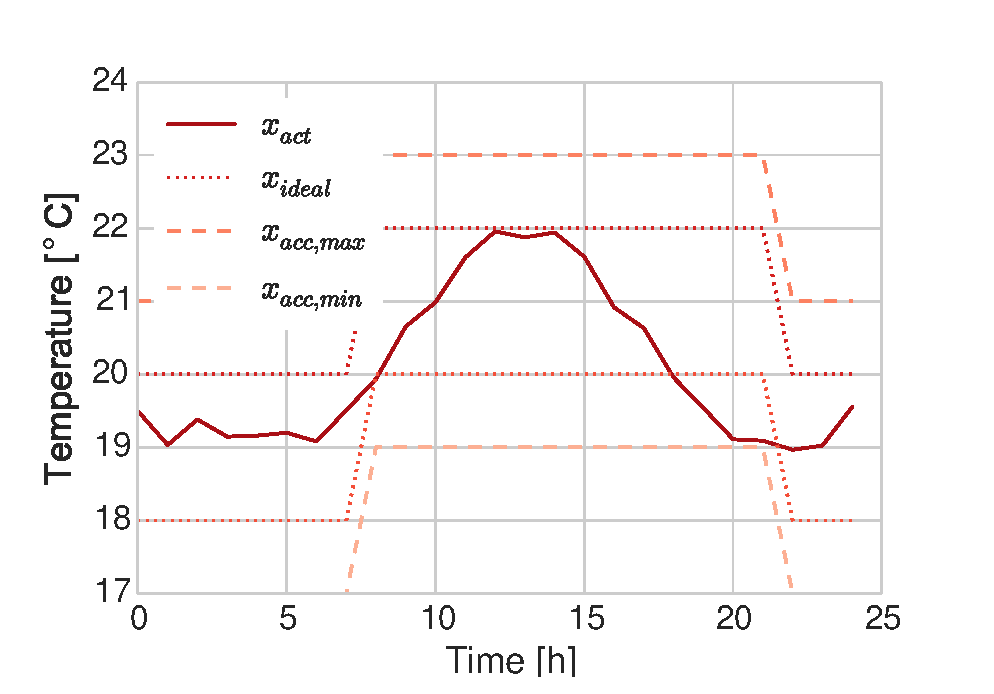
\includegraphics[width = \columnwidth]{SEGAN/tempband.eps}
\caption{Simulation of the indoor temperature of a Danish household.}
\label{fig:tempband}
\end{figure}

\begin{figure}
\centering
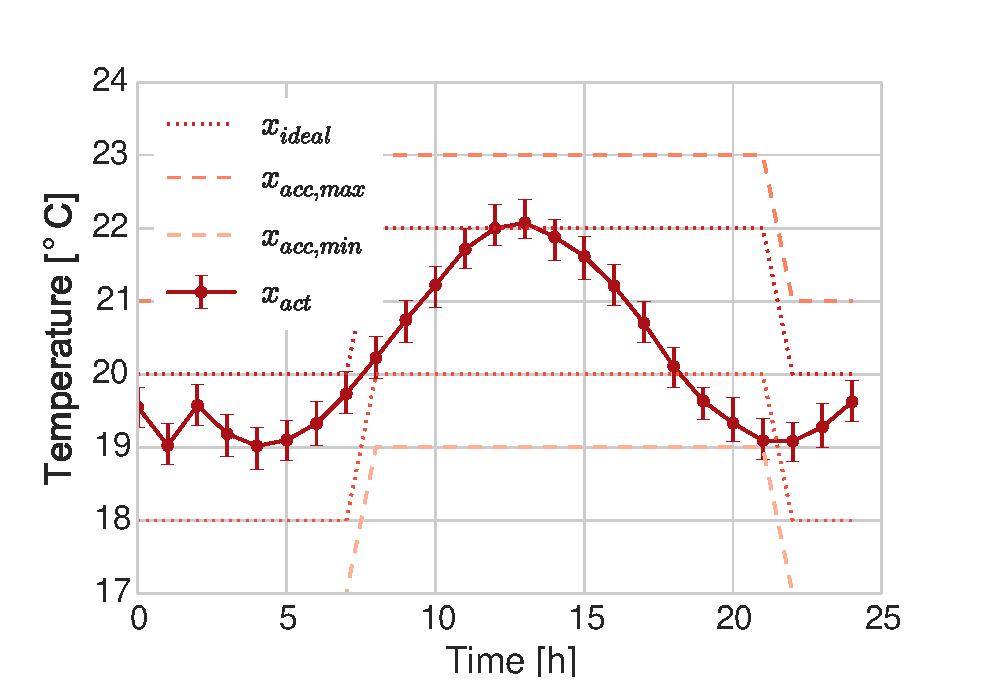
\includegraphics[width = \columnwidth]{SEGAN/tempbandclustererror.eps}
\caption{Simulation of the indoor temperature of 20 Danish households. The mean temperature is plotted, along with the minimum and maximum values of the cluster.}
\label{fig:tempbandclustererror}
\end{figure}


%\section{Previous section 4}
%\label{sec:newas}
%

%\begin{itemize}
%	\item Is it possible to avoid the baseline problem?
%	\item Define services in terms of performance, not characteristics.
%	\end{itemize}
%Product definition(suggestions):
%		\begin{itemize}
%			\item fast response product (gets paid for delivering in full as fast as possible, over short time horizons)
%			\item sustained delivery product (gets paid for the time period it is able to fully deliver the service)
%		\end{itemize}
% AS on the aggregators/DERs terms (new requirements)\\ 
%Verification and Settlement

\bondy{1) Ideal ancillary services needs are established and product performance is directly derived from these needs in form of a scalar heuristic based on performance variables. % are directly related to the system need. % (not upon minimum requirements).
2) remuneration based upon optimal value of the scalar heuristic.
3) New service definition leads to a new market clearing mechanism.}

The ideal source for ancillary service is one with ``unlimited capabilities in terms of response time, energy output, ability to frequently reverse their output, ability to respond and follow the AGC setpoint changes, and size .''\cite{makarov2008assessing}\footnote{For this kind of response to be optimal, changes must be made to the AGC algorithm \cite{peydayesh2012effects}.} In order to include and give incentive to the participation of technologies that in some parameters are closer to the ideal than those defined by the current service and market requirements, two methods can be utilized: product differentiation or product restructuring.

Some transmission system operators, like PJM, have already introduced the idea that better service performance is more valuable\footnote{See RegA and RegD in [cite].}, and split their regulation market into slow service product and a fast service product. 

This work explores the alternative, that is, restructuring the market, such that all technologies can participate in the same market, and the system operator can optimize the use of the resources based upon their capabilities. This entails reformulating the temporal and market requirements, and removing the requirements that implicitly assume that the services are provided by traditional generators, thus making the requirements technology agnostic.

The new service requirements definitions

- PRIM derived from inertia and no overshoot beyond settling frequency \& duration derived from secondary response \\
-- dimensioning of primary reserve defines settling frequency

- SECO derived from (cost/resource-optimal) primary and desired frequency restoration time 

- TERT derived from time to response

%It is concluded in \cite{makarov2008assessing} that a generator providing ancillary services close to the ideal (i.e. with large ramping rates), are more efficient for arresting frequency excursions earlier, and are therefore more valuable. There is a system wide benefit in creating better market opportunities for fast responsive resources. But in some instances, units that are able to provide very fast responses are not able to sustain their response for the currently required length of time (\textcolor{red}{refer to Vestas example if published, or other relevant example}).\bondy{To do: This whole paragraph should be reformulated so that the parameters are more generic, according to the service} Therefore the value of a unit should not only be evaluated based upon its ramping time, but also its response endurance. This paper proposes a new way of expressing these two service requirements into a single value. 

\subsection{Service Performance Parametrization}
Resource model: 

 - PROPOSAL1: ramp rate (MW/min), delay(min), duration (min), power (MW)\\
 
VOLUME:  (duration-(delay+power/ramp))*power+1/2*power/ramp*power)
 
- PERF: RMSE(Ideal unit parameters - parameters of the volume brick)
 
 - PROPOSAL2: full response time, duration, power\\
 
 alpha1*duration + alpha2*power - alpha3*

\bondy{We need express the system needs through parameters. Bring in Figure 3 or similar}\\
indicators

defining perfectly (responding) resource characterization

"threshold response" - the minimally acceptable reserve provisions (the reserve need)



\subsection{Performance-based Remuneration}

\subsection{Service Procurement Process}
\textit{Step 1:} Ancillary service specification by System operator. A system operator defines the system requirements and objectives for a specific ancillary service. These requirements are primarily formulated in terms of minimum requirements for the overall response. 

\textit{Step 2:} (AS) Service tender conditions: 
The tender defines requested total service volume, bid parameters and a derived performance parameter $\kappa$. 

The bid parameters are service-specific and serve both for market-clearing and performance calculation. The parameters are chosen considering idealized response characteristics, simplicity of calculations, service needs, verifiability, (linearity?) \kh{[...tbd...] }
The performance parameter defines the trade-off between bid parameters. 

Also, the tender will specify the granularity of the bids, so there is a standard bid size, e.g. 1 kW, of which each player can bid several of. For example, if aggregator \emph{X} wants to sell 5 MW, it bids 5000 units of the service. In this way, each bid's performance value $\kappa$, and the parameters that conforms it, will be comparable.

Steps 1-2 apply define the market setup. Steps 3-7 apply to each tendering period. 

\textit{Step 3:} Bid formulation:
AS aggregator bids submitted include: 
\begin{itemize}
\item offered service parameters
\item bid price
\item (for cross-validation) estimated $\kappa$
\item unit quantity (volume)
\end{itemize}


\textit{Step 4:} Market Clearing: based on submitted bids and required procurement volume the market is cleared by incrementally increasing the pool. For each new block of bids added to the portfolio, a new tetris optimization is done by the TSO. When the minimum requirements to the service specifications is met, the market is finished/cleared.

outcome: procured reserve portfolio; market clearing price according to the highest cleared price.

[\textit{Step 5: }Activation]

[\textit{Step 6:} Verification]

\textit{Step 7:} Remuneration is based on the market clearing price and the performance parameter $\kappa$. 
$\$*volume * \kappa - penalty$
penalty if Bid specs not met according to validation.


\textit{rationale:} \\
a) clearing at marginal cost provides correct competitive incentives [cite?Nordic market]; 

b) removal of 'minimum' requirements facilitates market liquidity, removing barriers for demand response participation;

c) performance-based remuneration favours better service \kh{[ahrr -this is so obvious, i can't find the words]};

d) bid formulation uses simplified constraints that can be addressed both for conventional generation and are also straightforward to be formulated as response capability of a diverse DR portfolio;

e) Steps 5 \& 6 out of scope/do not require revision.




\subsection{Proposal for Market Structure and Clearing}

In order to clear the market, all bids are sorted into a merit order list (price vs. volume), and the TSO will select from cheapest to most expensive the bids that covers its needed spectrum of $\kappa$ values. \kara{I don't think $\kappa$ is introduced before.}

%At the same time, demand response (DR) has shown to be capable of very fast ramping times \textcolor{red}{[cite:Vrettos-Powertech,Changhong Zhao-Caltech (Jason attended his talk) others?...]} which leads to arresting frequency excursions faster and at higher nadir. But for the foreseeable future traditional generators will still be delivering most of the ancillary services, and therefore the requirements must encompass the capabilities of both both slow reacting and fast reacting units. We therefore propose that the performance requirements are defined as a band, where the lower bound is the minimum acceptable service delivery, and the upper bound is represented by the optimal (hence by definition the maximum achievable) response.

%There are few of the current requirements that already measure performance (Table~\ref{tab:requirements}).% For primary frequency control, the change in operating point according to the frequency deviation $\Delta_P$, as well as the controller insensitivity (dead-band) are two parameters that describe the performance of the service.


%Definition of services in term of the droop dead-band and the shape of the slopes of the droop.
%
%Requirements that make sense:
%\begin{itemize}
%\item Primary frequency control
%\begin{itemize}
%\item Dead band
%\item Full delivery within \emph{x} time (could be a curve as proposed by Eto)
%\item ``droop'' (call it something different)
%\end{itemize}
%\begin{itemize}
%\item Deployment start
%\item Full delivery/availability
%\end{itemize}
%\end{itemize}
%
%I propose, to use the Integral Square Error index (as in my ISGT paper) and define the requirements as minimum and optimal bands. Depending on how we define the error, the quadratic nature of the ISE will emphasize punishment of performance close to the acceptable limits, or emphasize reward of performance close to the ideal.

%\begin{equation}
%\Delta P_G(t) = - \frac{1}{f_n S_G}\Delta f_m (t) P_{G,n}.\label{eq:droop}
%\end{equation}
%For primary frequency response, the optimal response is formulated from the optimal droop, following the equation:
%and the frequency dead-band. The minimum response requirement is given in base of the how long the generator has to give the maximum output (established by Eq.~\eqref{eq:droop}). Also, a probabilistic term could be added, such that 95 percentile respects the requirements. The response would be a linear transformation of the frequency deviation (Figure~\ref{fig:primarydroopresponse})
%\begin{figure}[ht!]
%\centering
%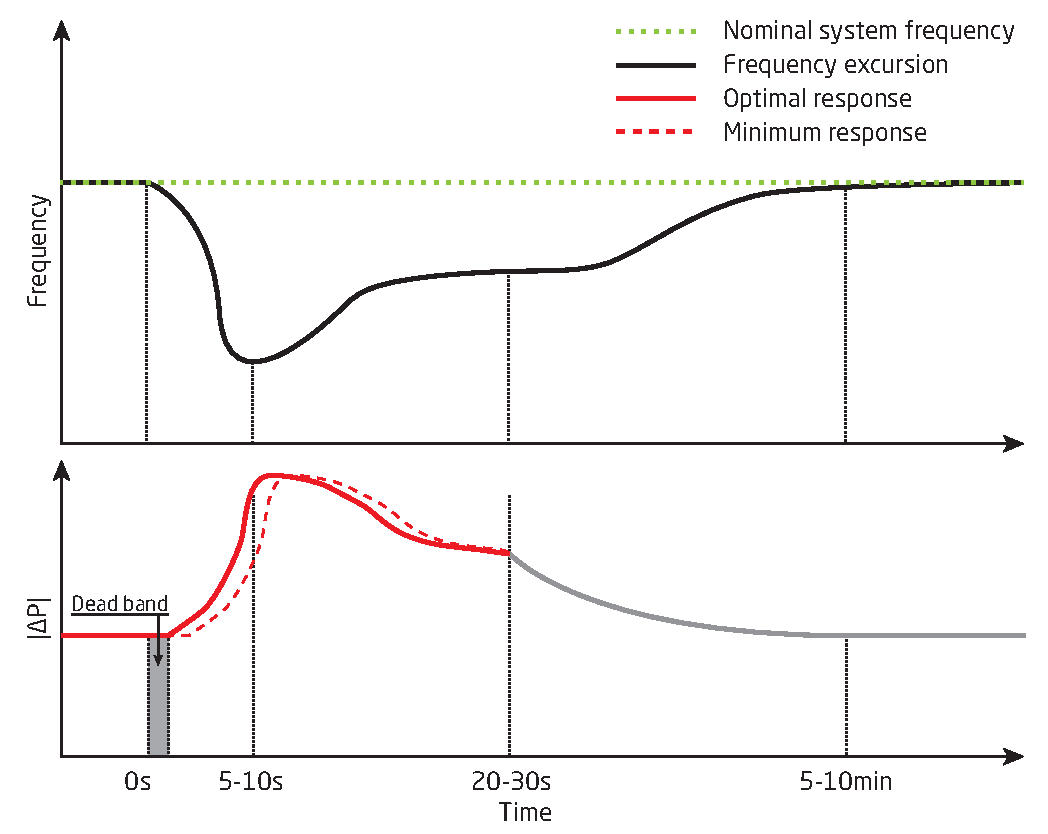
\includegraphics[width=1\columnwidth]{primary_frequency_control.pdf}
%\caption{Power response of a primary frequency control providing unit with perfect frequency following and with a droop of 4\%.}
%\label{fig:primarydroopresponse}
%\end{figure}
%
%Another way of formulating the optimal response is in terms of the rise time of the response (Figure~\ref{fig:primarytimeresponse})\cite{eto2010use}.
%\begin{figure}[ht!]
%\centering
%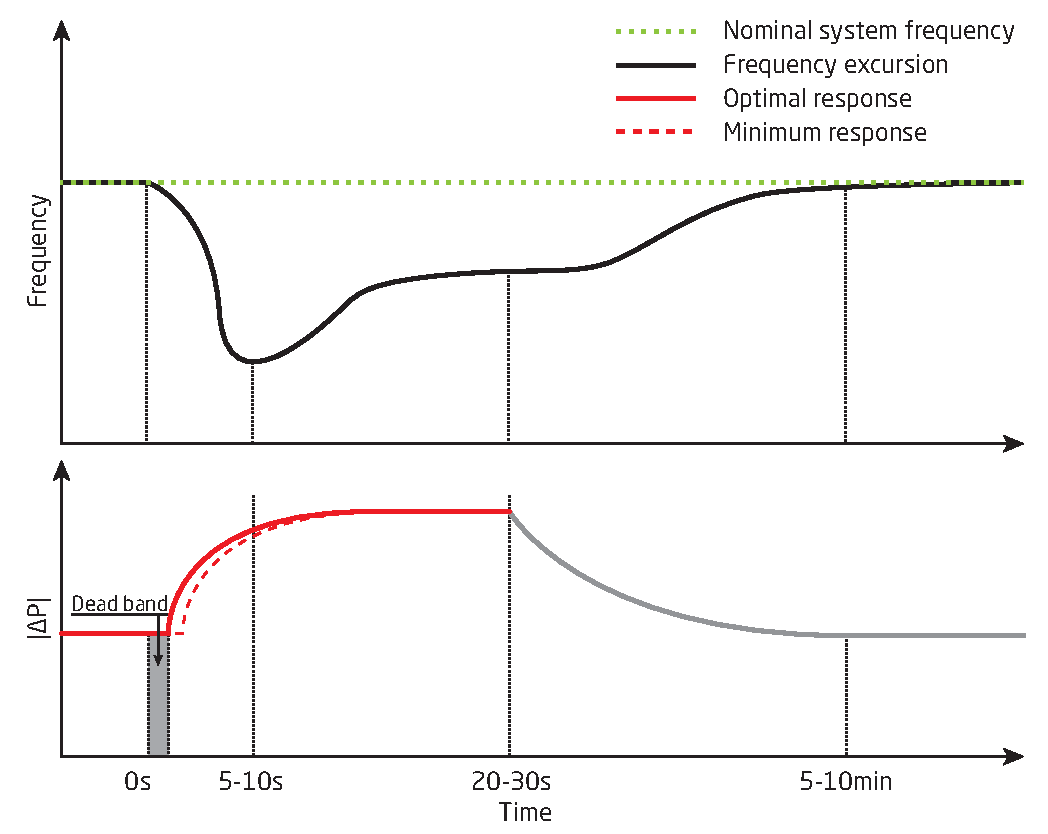
\includegraphics[width=1\columnwidth]{primary_frequency_control2.pdf}
%\caption{Power response of a primary frequency control providing unit when full delivery must be achieved within a time frame.}
%\label{fig:primarytimeresponse}
%\end{figure}
%
%For the secondary frequency control, the optimal response is formulated as a step function, or near step function because a response that is too steep could cause system instability. As in primary frequency control, the limits are defined by the allowable delay and a probabilistic term (Figure~\ref{fig:secondarytimeresponse}).
%\begin{figure}[ht!]
%\centering
%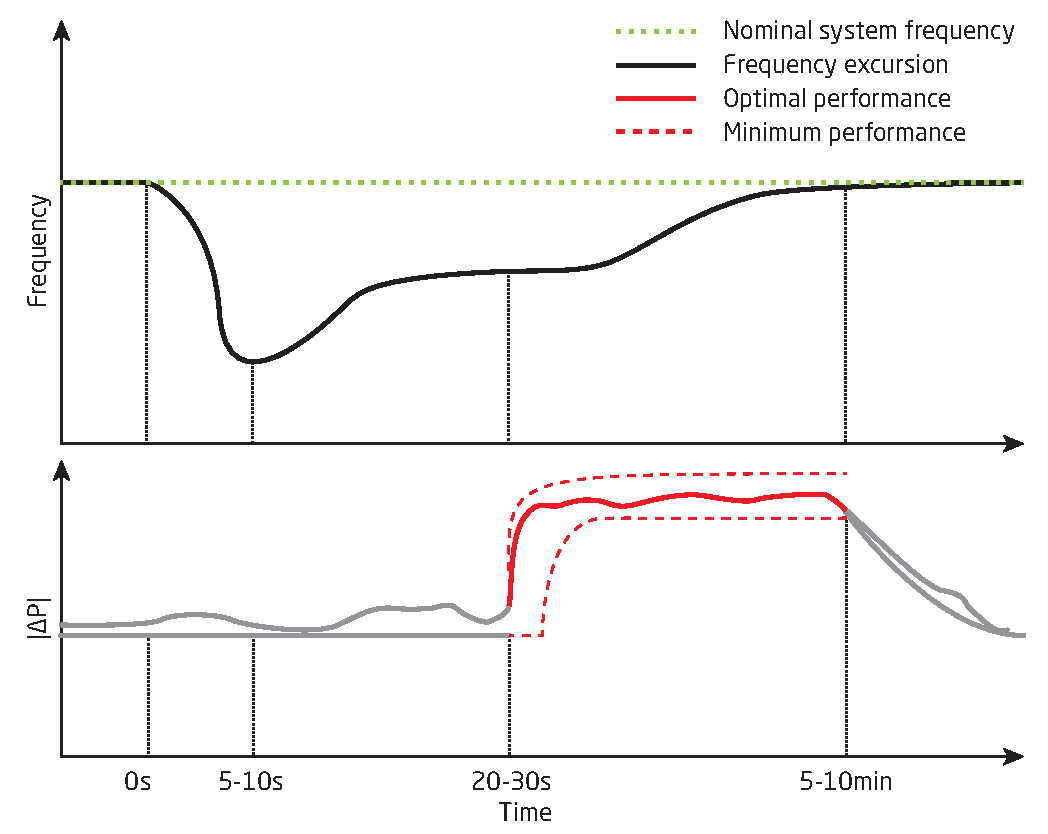
\includegraphics[width=1\columnwidth]{secondary_frequency_control2.pdf}
%\caption{Power response of a unit providing secondary frequency control indicating a time frame in which full delivery must be achieved.}
%\label{fig:secondarytimeresponse}
%\end{figure}
%We have identified three categories of requirements for ancillary services: performance requirements, unit specification requirements and market requirements.
%
%For primary frequency control the classification is the following:
%
%\emph{Performance requirements:} 
%\begin{itemize}
%\item Full availability
%\item Deployment end *
%\item Frequency characteristic
%\end{itemize}
%
%\emph{Unit specification requirements:}
%\begin{itemize}
%\item Droop of generator
%\item Compulsory adjustable droop
%\item Accuracy of frequency measurements
%\item controller insensitivity
%\item full deployment before a deviation of \emph{X} frequency
%\item Accuracy of SCADA measurements **
%\end{itemize}
%
%\emph{Market specification requirements:}
%\begin{itemize}
%\item Minimum reserve/bid size
%\item Contract \emph{X} time before delivery
%\item Bid symmetry
%\item Combined delivery
%\end{itemize}
%
%For secondary frequency control the classification is the following:
%
%\emph{Performance requirements:} 
%\begin{itemize}
%\item Deployment start
%\item Full availability
%\item Deployment end *
%\end{itemize}
%
%\emph{Unit specification requirements:}
%\begin{itemize}
%\item Control architecture
%\item Accuracy of frequency measurement
%\item Exchanges measurement
%\item Controller cycle time
%\item Controller type (P-term and I-term if applicable)
%\item K-factor for measuring ACE
%\item Accuracy of SCADA measurements **
%\end{itemize}
%
%\emph{Market specification requirements:}
%\begin{itemize}
%\item Minimum bid size
%\item Contract \emph{X} time before delivery
%\item Bid symmetry
%\item Combined delivery
%\item Bid duration
%\end{itemize}
%
%For tertiary frequency control the classification is the following:
%
%\emph{Performance requirements:}
%\begin{itemize}
%\item Deployment start
%\item Full availability
%\item Deployment end\textcolor{red}{(not sure on this one, since in many cases it is a rescheduling)}
%\end{itemize}
%
%\emph{Unit specification requirements:}
%\begin{itemize}
%\item Accuracy of SCADA measurements **
%\end{itemize}
%
%\emph{Market specification requirements:}
%\begin{itemize}
%\item Minimum bid size
%\item Contract \emph{X} time before delivery
%\item Bid symmetry
%\item Combined delivery
%\item Bid duration
%\end{itemize}

\section{Case Study}
\label{sec:casestudy}
Using two different ancillary services and an asset management service as cases, we will illustrate the utility of the generic service modeling method, the service performance index and the service verification index. The first case study focuses on frequency containment reserve in western Denmark, the second focuses on the theoretical PowerMax DSO service, and the third focuses on the temperature management of a residential house. 

\subsection{Frequency Containment Reserve in Western Denmark}
Frequency Containment Reserve (FCR) is utilized to contain frequency excursions deviating from the nominal 50 Hz in \emph{ENTSO-E RG Continental Europe’s synchronous area} of which western Denmark (DK1) is part of. The Danish TSO, Energinet.dk, is obliged to provide a proportional share of $\pm$ 23 MW \cite{EnerginetAncillary} out of the total synchronous area need of $\pm$ 3000 MW. Energinet.dk buys these reserves at daily auctions. The service specifications are defined in \cite{EnerginetAncillary}.

The six steps outlined in Sec.~\ref{sec:SEGANmethodology} are used to model the ideal and tolerated service response. 1) The physical parameters are grid frequency (accuracy of $\pm$ 10 mHz or better), generator reserve power output, and timing of service delivery (accuracy of 1 s or better). 2) The reserve must be supplied linearly at deviations of $\pm$ 200 mHz relative to 50 Hz, with a $\pm$ 20 mHz dead-band around 50 Hz. 3) The physical size of the service depends on the reserve bid size. This work will look at a generic reserve bid. According to the discussion from Eq.~\eqref{eq:QoS}, $x_{ideal}$ cannot be equal to $\mathbf{x}_{acc}$. Therefore, a $\pm$ 1\% tolerance band of $x_{ideal}$ is assumed. 4) The first 50\% of the service must be supplied within 15 s and 100\% must be supplied within 30 s. The ideal response can be defined as a response with an instant 100\% power ramp \cite{makarov2008assessing}. 5) The ideal and tolerated response of this service provision is plotted as $x_{ideal}$, $x_{acc,min}$ and $x_{acc,max}$ in Fig.~\ref{fig:DK1PrimResSim}, which assumes that a reserve power set-point has already been established based on the values from step 2.%Fig.~\ref{fig:DK1PrimResDyn}

%\begin{figure}
%\centering
%\includegraphics[width=\columnwidth]{figures/dynresp.eps}
%\caption{DK1 Primary Reserve service provision curve. The curve shows the relationship between the activated fraction of the primary reserve bid, and the grid frequency, including the +/- 20 mHz dead-band. This should not be confused with the droop curve.}
%\label{fig:DK1PrimResDyn}
%\end{figure}

Fig. \ref{fig:DK1PrimResSim} shows a simulation of primary regulation active power ramp $x_{act}$ for the time interval $[-5,35]$ s. The service delivery performance index and non-delivery verification index are $\eta^{AS}=0.4257$ and $\epsilon^{AS}=0.1392$, calculated using Eq. \eqref{eq:etaAS} and Eq.~\eqref{eq:epsilonAS}. The TSO must determine a threshold $\epsilon_{max}$, such that the service provider is penalized or the contract is terminated if $\epsilon^{AS}>\epsilon^{AS}_{max}$. It is not the scope of this work to asses a suitable value of $\epsilon^{AS}_{max}$.%\bondynote{We are repeating ourselves a bit here}

\begin{figure}
\centering
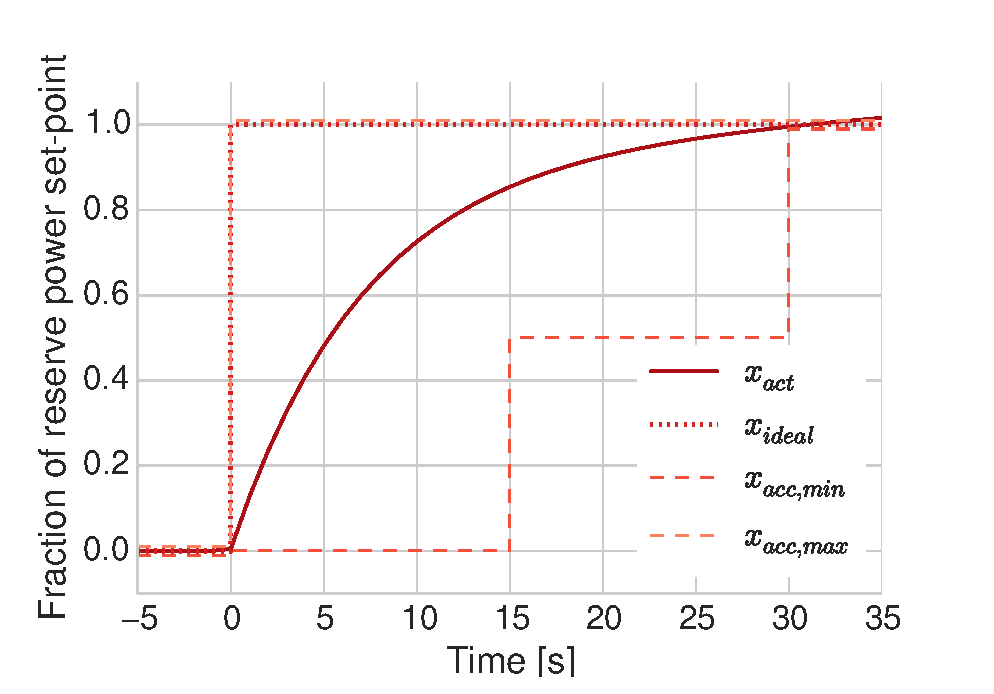
\includegraphics[width = \columnwidth]{SEGAN/primfreqresp.eps}
\caption{Simulation of a DK1 primary reserve power ramp response together with $x_{ideal}$ and $x_{acc}$ values.}
\label{fig:DK1PrimResSim}
\end{figure}

\subsection{PowerMax in a distribution system}
The \textit{PowerMax} service was first described in \cite{ding2013development} and further specified in \cite{bondy2014flech}. It is a DSO service, where the DSO can make a tender for a load reduction $\Delta P^{DSO}$ to a max level $P_{max}^{DSO}$ in parts of the distribution system that are forecasted to experience congestions during some periods (e.g. hours 17-20 during winter months). The motivation for \textit{PowerMax} is that the service could be an economically beneficial alternative to grid reinforcements in some situations. This is both due to saved interest and depreciation on investments plus the avoided risk of over-sizing equipment in case of future energy savings or if the disappearance of a large consumer makes the reinforcement unnecessary.% The tender is announced and cleared through Flexibility Clearing House (FLECH), where flexibility aggregators can bid on the tender.%where the service is delivered by aggregator companies, which bid in flexibility from a group of units which they control. 

%Following is a mathematical definition of the \textit{PowerMax} service, as previously developed in \cite{bondy2014powermax}. 
In order to identify its service needs, it is assumed that the DSO is able to separate the total consumption forecast $\hat{P}_{tot}$ in the congested part of the distribution grid into a controllable load forecast $\hat{P}_{CL}$ and a base load forecast $\hat{P}_{BL}$:
\begin{align}
\hat{P}_{tot} &= \hat{P}_{CL} + \hat{P}_{BL} \\
\hat{P}_{CL} &= \sum_{Agg} \hat{P}_{CL,Agg}, \quad Agg \in \mathbf{A} \label{eq:CLDef}
\end{align}
where $\mathbf{A}$ is the set of all aggregators in the considered part of the grid. Only the aggregators \emph{Agg} that bid for the service tender make up $\hat{P}_{CL}$, while the rest of $\mathbf{A}$ is part of $\hat{P}_{BL}$. The aggregators must be contracted to deliver a total power reduction $\Delta P$, such that the system operational limit $\bar{P}_{sys}$ is not violated by the peak base load forecast and the peak controllable load forecast:

\begin{equation}
\hat{\bar{P}}_{BL}+\hat{\bar{P}}_{CL}-\Delta P \leq \bar{P}_{sys}. \label{eq:PSysDef}
\end{equation}

This inequality can be fulfilled by setting a peak limit $\bar{P}_{CL}$:
\begin{equation}
\bar{P}_{CL} = \hat{\bar{P}}_{CL} - \Delta P \label{eq:PBarCLDef}
\end{equation}
where $\Delta P$ and $\bar{P}_{CL}$ are the variables for the DSO service tender. In order to formulate a service tender, the magnitude of these variables must be estimated taking into account the uncertainty of the forecasts, giving the following expressions:
\begin{align}
\Delta P^{DSO} &= \sum_{Agg} \Delta \hat{P}_{CL,Agg} + \text{Risk\{}\hat{P}_{CL} + \hat{P}_{BL}\text{\}}\\
P_{max}^{DSO} &= \hat{\bar{P}}_{CL} - \Delta P_{DSO}
\end{align}
where $\Delta \hat{P}_{CL,Agg}$ is the estimated power reduction for the individual aggregator bid, $\text{Risk\{}\hat{P}_{CL} + \hat{P}_{BL}\text{\}}$ is the risk associated to the load forecast uncertainty. $Agg \in \mathbf{A_{C}}$ and $\mathbf{A_{C}} \subseteq \mathbf{A}$, i.e. $\mathbf{A_{C}}$ is the subset of aggregators that bid on the tender. After the DSO has identified a suitable $P_{max}^{DSO}$ and $\Delta P^{DSO}$ to solve the congestion issue, the DSO formulates a service tender for which aggregators can bid their corresponding $\Delta P^{Agg}$ and $P^{Agg}_{max}$. %The DSO sets a maximum price it is willing to pay for the load reduction, which is related to the alternative cost of grid reinforcements. In case the market is not cleared at or below the maximum price, the DSO can formulate a new tender, adjusting the risk value, POD (point of delivery) list or amount of power reduction. The timing of the tender process should be such that the DSO has time to conduct grid reinforcements as an alternative.

The method from Sec.~\ref{sec:SEGANmethodology} is used to model \textit{PowerMax} ideal and acceptable response. 1) The physical parameters are $P_{max}^{Agg}$, $\Delta P^{Agg}$ and months/days/hours the service shall be delivered. 2) The system does not posses a dynamic behaviour related to system parameters. 3) As an example, the service tender defines $P_{max}^{Agg} = 200$ kW and $+1\%$ allowed deviation $P_{max,acc}^{Agg}$. 4) In this example we use 120 min service provision time with allowed non-delivery in the first 15 min, and the last 5 min, of the service delivery (following the service definition in \cite{ding2013development}) and the ideal service delivery is the one that respects $P_{max}^{DSO}$. 5) Figure \ref{fig:PowerMaxSim} plots $x_{ideal}$ and $x_{acc}$. The \textit{Activation Dead-band} indicates the regions where the aggregator is not obliged to deliver the service because of the tolerances defined under step 4. 6) The service is a maximum cap service and the error is measured as in Eq.~\eqref{eq:maxmin_cap}.

An example of a load curve $P_{Agg}=x_{act}$ is presented in Fig.~\ref{fig:PowerMaxSim}. The service delivery and verification are evaluated using Eq.~\eqref{eq:etaAS} and Eq.~\eqref{eq:epsilonAS}, yielding $\eta^{AS} = 0.5074$ and $\epsilon^{AS} = 0.2701$ respectively. As with the performance assessment of the FCR in DK1, it is not within the scope of this paper to asses the value of $\epsilon^{AS}_{max}$, yet a qualified assessment can be made. %, which will lead to either penalization or termination of the contract.
To asses $\epsilon^{AS}_{max}$, the DSO must analyze the dynamics of the problem the service is helping relieve. For \textit{PowerMax}, the dynamics are governed by the heating of the overloaded equipment (e.g. transformer or cable), which deteriorates over time due to overheating. A feeder might be tolerant to short term overloads and therefore the DSO might set $\epsilon^{AS}_{max}$ higher than in the FCR case.

\begin{figure}
\centering
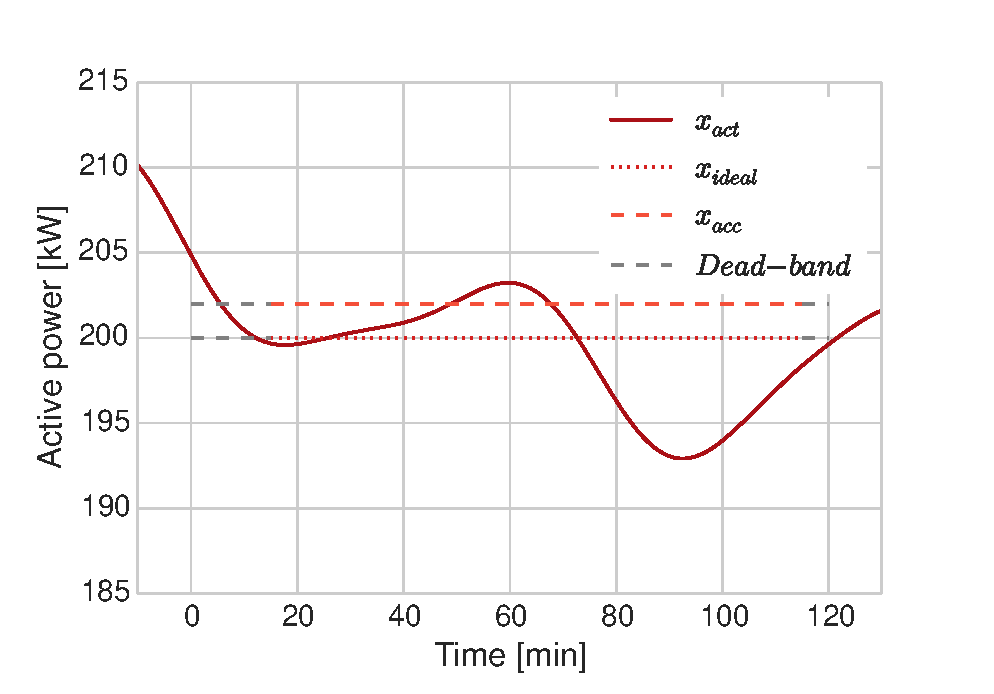
\includegraphics[width = 0.86\columnwidth]{SEGAN/powermaxsample.eps}
\vspace{-4pt}
\caption{$x_{ideal}=P_{max}^{Agg}$, $x_{acc}=P_{max,acc}^{Agg}$ for the considered \textit{PowerMax} example. The activation Dead-band is the time period, where the aggregator is allowed to non-deliver.}\label{fig:PowerMaxSim}
\end{figure}

\subsection{Temperature management of a flexible household}
Household heating is a flexible process where the thermal capacity of the building can be considered a form of energy storage. In Denmark, heat pumps are being installed with the capability of being remotely controlled by an aggregator, see e.g. \cite{insero}. It is assumed that the aggregator will help the heat pump owners to maintain a comfortable indoor temperature and utilize the electric consumption flexibility in exchange of monetary compensation.

Applying the method from Sec.~\ref{sec:SEGANmethodology} to model the service: 1) The physical parameters are the minimum and maximum of the temperature comfort bands of the household. 2) The service does not posses a dynamic behaviour related to system parameters. 3) As an example, the household owner sets a comfort band of $\mathbf{x}_{ideal} = [x_{min},x_{max}] = [20 ^{\circ}\text{C},22^{\circ}\text{C}]$ and allows for a $\pm 1 ^{\circ}\text{C}$ as acceptable error. Furthermore, the owner decides that during the night, the house can be two degrees colder. 4) In this example the ideal response is performance within the temperature bounds. 5) Fig.~\ref{fig:tempband} plots $x_{ideal}$ and $\mathbf{x}_{acc}$. 6) The service is a band service and the error is measured according to Eq.~\eqref{eq:band_error}.

The service model and the actual temperature of a simulation can be seen in Fig.~\ref{fig:tempband}, where it is clear that generally the aggregator is able to provide a reasonable service performance, with no non-delivery ( $\eta^{AMS} = 0.2707$ and $\epsilon^{AMS} = 0.0$). As described in Sec.~\ref{sec:DERs}, the aggregator may be in charge of the overall control of a cluster of units, in which case the performance should be evaluated over the whole cluster. To show this, simulations are done for 20 households and the equally-weighted average of the indices results in $\eta^{AMS} = 0.2411$ and $\epsilon^{AMS} = 0.0211$ (Fig.~\ref{fig:tempbandclustererror}).

\begin{figure}
\centering
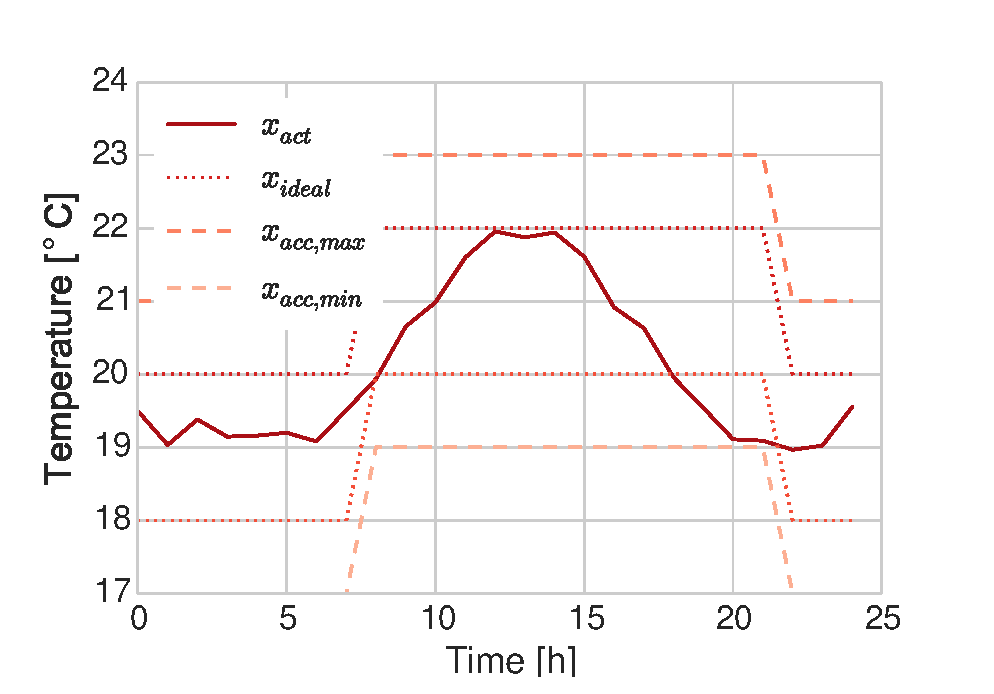
\includegraphics[width = \columnwidth]{SEGAN/tempband.eps}
\caption{Simulation of the indoor temperature of a Danish household.}
\label{fig:tempband}
\end{figure}

\begin{figure}
\centering
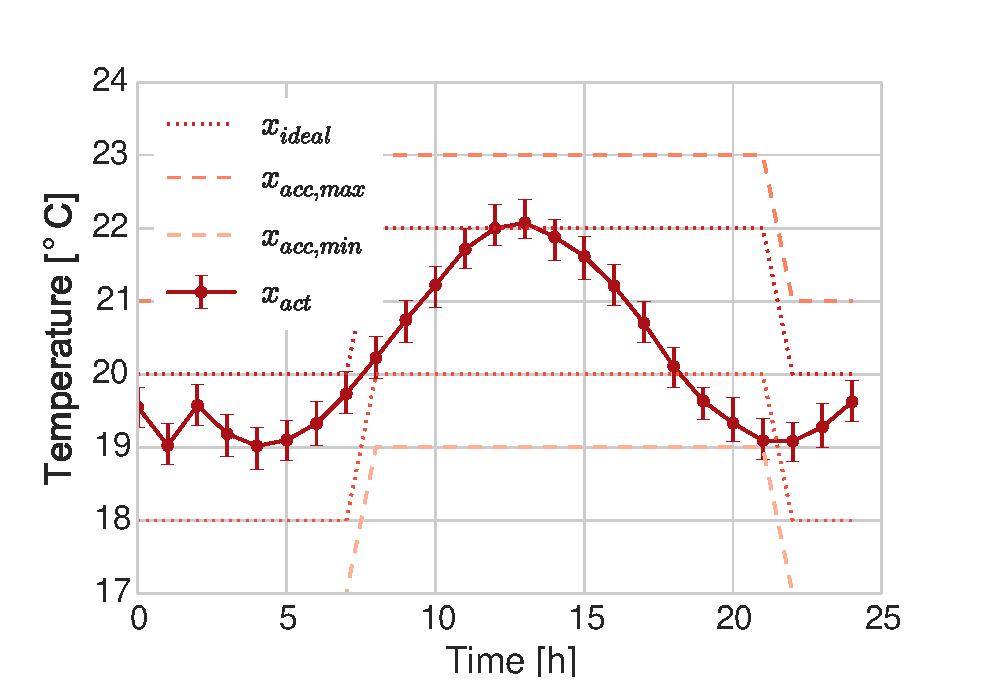
\includegraphics[width = \columnwidth]{SEGAN/tempbandclustererror.eps}
\caption{Simulation of the indoor temperature of 20 Danish households. The mean temperature is plotted, along with the minimum and maximum values of the cluster.}
\label{fig:tempbandclustererror}
\end{figure}


\section{Discussion}
\label{sec:discussion}
\section{Discussion}
Specific terminology has been introduced to describe the proposed method. This terminology can be mapped to that of the field of \emph{Design of Experiments}, e.g. \emph{definition of service requirements} maps to \emph{definition of inner-noise factor} and \emph{definition of test inputs} maps to \emph{definition of outer-noise factors}. Specifically, the method resembles \emph{fractional factorial methods for off-line quality control}, see e.g.\cite{oehlert2010first}. In the case study presented in Sec.~\ref{sec:casestudy}, the inner factor, or controllable variable, is kept at a single level, i.e. the same activation signal is sent to the aggregator for each run of the experiment. The two outer factors, or noise variables, were varied over a distribution dictated by the operational scenario, i.e. the availability of the portfolio was varied on seven levels and, likewise, the process noise in the house simulation models was varied on seven levels. An important contribution of this work is applying this kind of formal test procedures to the problem of aggregator validation. The field of Design of Experiments is broad, and a further revision on the topic may yield a better method proposals than the one proposed here.

In this paper we focus only on the two  uncertainty sources mentioned above, therefore the test for time responsiveness, i.e. delay in the communications systems between the aggregator and a DER is not considered. This means that the test design presented in the case study is a simplified version of what an actual aggregator validation test would require. Future research must identify the relevant variables that need to be tested under the relevant operation scenarios. 

In comparison with the traditional test method, this validation procedure must capture the capabilities of a much more complex system, and therefore relies in part on simulations. As presented in \cite{steinbrink2015challenges}, the error between the used models and reality must be quantified and taken into account for the final aggregator certification. Each block in the simulation must use validated models or software. This applies to the communication systems, the grid models and the DER models. The test architecture, e.g. the one presented in \cite{buscher2015towards}, which validates the aggregators must also be validated.

There are still several open issues that need to be investigated with regards to aggregator validation. For example, the definition of the operation scenarios was only briefly discussed, and heuristics must be developed in order to define scenarios that are effective when testing aggregators.

Aggregator validation must be an ongoing process, that should be carried out periodically or whenever the aggregator portfolio or architecture changes significantly. Furthermore, aggregators are expected to participate in different electricity markets. Due to these reasons, along with the complexity of designing appropriate simulations, we believe that the task of validating aggregators should not carried out by the system operators, but by an independent third party. 

\section{Conclusion}
\label{sec:conclusion}
\section{Conclusion and Future Work}
This work presents an initial approach to establishing a methodology for designing aggregator validation tests. This method differs from the traditional generator certification tests in that it must be carried out in simulations, so that the stochasticity of the real world disturbances affecting the aggregator can be taken into account. A drawback of this method is that it relies on the accuracy and complexity of the simulation models. This means that the components of the validation tests must be validated against reality. The test method was shown through a simplified case study on an existing aggregator. While the example shows a fictive TSO applying the test to a fictive aggregator, there is the possibility that validation of aggregators in the future will be carried out by third party test companies. 

There are still several open issues that need to be investigated with regards to aggregator validation. For example, the definition of the operation scenarios was only briefly discussed, and heuristics must be developed in order to define scenarios that are effective when testing aggregators.

An important step for the development of the validation method is the implementation of a complete test architecture with validated component models. With such a simulation framework, with realistic communication and DER models, communication delays can be implemented in order to test aggregators for time responsiveness. 

Finally, the method should be expanded to cover other ancillary services, such as voltage regulation.

We consider the work presented here an important element of enabling aggregators in the smart grid, thus enabling consumption to actively participate in the secure operation of the power system. This will help the integration of renewable energy sources into the power system.

\section*{Acknowledgments}
We're going to ask for feedback from:
\begin{itemize}
	\item John Goodin (CAISO)
	\item Paul Wattles (ERCOT)
	\item Donna Pratt (NYISO)
	\item Scott Baker (PJM)
	\item Joe Eto (LBNL)($\surd$)
	\item EirGrid (through Mark O'Malley)
	\item Energinet.dk (Preben Nyeng? Peter Bruhn)
\end{itemize}
\bibliography{references/library.bib}{}
\bibliographystyle{ieeetr}
\end{document}


